\documentclass[11pt,dvipsnames]{article} % {{{

\usepackage{geometry}
\geometry{total={170mm,240mm}, left=20mm, top=20mm}

\usepackage[utf8]{inputenc}
\usepackage[english]{babel}
\usepackage{physics} 
\usepackage{siunitx} 
\usepackage{enumerate} 
\usepackage{pgfplots}

% Ubicación imágenes
\usepackage{graphicx}
\graphicspath{ {./images/} }

\usepackage{subcaption}
\definecolor{mycolor}{RGB}{255,50,0}

\usepackage{pgfplotstable}
\usepackage{tikz,pgfplots}
\usepackage{amsmath} 
\usepackage{xcolor}
\usepackage{float}
\usepackage{amsfonts}
\newcommand{\pce}{PCE}
\usepackage{dsfont}

\newtheorem{conj}{Hypothesis}


\newcommand{\fref}[1]{fig.~\ref{#1}}  
\newcommand{\tref}[1]{table~\ref{#1}}
\newcommand{\Fref}[1]{Fig.~\ref{#1}}  
\newcommand{\Tref}[1]{Table~\ref{#1}}

\newcommand{\R}{\mathcal{R}}
\newcommand{\psii}{\psi_i}
\newcommand{\Pk}[1]{\ket{\psi_{#1} }}
\newcommand{\Pb}[1]{\bra{\psi_{#1} }}
\newcommand{\pk}{\ket{\psi}}
\newcommand{\M}{\mathcal{M}^{(N)}}
\newcommand{\E}{\mathcal{E}}
\newcommand{\Ej}[1]{\E_{j_{#1}}}
\newcommand{\id}[1]{\qty(\1-\E_{j_{#1}})}
\newcommand{\Erho}{\mathcal{E}(\rho)}
\newcommand{\1}{\mathds{1}}
\newcommand{\ten}{\otimes}
\newcommand{\h}[1]{\colorbox{Yellow}{#1}}
\newcommand{\hi}{\mathcal{H}}
\newcommand{\txt}[1]{\text{#1}}
\newcommand{\here}{\h{\hspace{15cm}} }
\newcommand{\rhoi}{\dyad{\psii}{\psii}}
\newcommand{\ind}[2]{ {{}^{#1}_{#2}} }
\newcommand{\rc}[1]{r_{#1}}
\newcommand{\pauli}[2]{\sigma_{#1}\otimes\sigma_{#2}}
\newcommand{\Er}{\E_{\mathcal{R}} }
\newcommand{\PCE}[1]{\mathsf{PCE}_\mathsf{#1}}
\newcommand{\ot}{\otimes}

\usepackage{imakeidx}
\makeindex[columns=3, title=Alphabetical Index, intoc]


%\usepackage[]{lineno}  \linenumbers
%\setlength\linenumbersep{3pt}

\usepackage{fancybox}
\usepackage{colortbl}
\usepackage{amsbsy}
\usepackage[draft,inline,nomargin]{fixme} \fxsetup{theme=color}
\FXRegisterAuthor{cp}{acp}{\color{blue}CP}
\FXRegisterAuthor{ja}{aja}{\color{mycolor}JA}
\FXRegisterAuthor{dd}{ddg}{\color{red}DD}

\title{Pauli component erasing operations} 

% }}}
\begin{document}
% Titulo y otros {{{
\maketitle
\tableofcontents
% }}}

\section*{Carlos' ideas}
\section{CP from eigenvalues} % {{{
% Intro {{{
Choi matrix's eigenvalues of a 1-qubit Pauli Channel are
\begin{align}
\lambda_{\mu}=1+\sum_{j=1}^3a_j^{\mu}\tau_j
\hspace{35pt}
\mu=0,1,2,3;
\hspace{35pt}
a_j^{\mu}=\left\{ \begin{array}{rl}
             1, & \mu=j \lor \mu=0\\
             -1, & \mu\neq j
             \end{array}
   \right..
\end{align}
Therefore, the inequalities needed to be sattisfied for a 1-qubit 
unital Pauli channel in order to be CP may be expressed in the 
following compact expression:
\begin{equation}
\sum_{j=0}^3a_j^{\mu}\tau_j\geq -1,
\hspace{35pt}
\mu=1,2,3;
\hspace{35pt}
a_j^{\mu}=\left\{ \begin{array}{rl}
             1, & \mu=j\\
             -1, & \mu\neq j
             \end{array}
   \right..
\end{equation}

Now, Choi matrix's eigenvalues of an n-qubit Pauli Channel are
\begin{align}\label{eq:eigvals-PCE}
\lambda_{\mu_1,\ldots,\mu_n}=1+
\sum_{\underset{(j_1,\ldots,j_n\neq0)}{j_1,\ldots,j_n=0}}^3
a_{j_1}^{\mu_1}\ldots a_{j_n}^{\mu_n}\tau_{j_1,\ldots,j_n}
\hspace{35pt}
\mu_l&=0,1,2,3,\nonumber\\
a_{j_l}^{\mu_l}&=\left\{ \begin{array}{rl}
             1, & \mu_l=j_l \lor j_l=0\lor \mu_1,\ldots,\mu_n=0\\
             -1, & \mu_l\neq j_l
             \end{array}
   \right..
\end{align}

Therefore, the inequalities needed to be sattisfied for the CP are
\begin{equation}\label{eq:inequalities-PCE}
\sum_{\underset{(j_1,\ldots,j_n\neq0)}{j_1,\ldots,j_n=0}}^3
a_{j_1}^{\mu_1}\ldots a_{j_n}^{\mu_n}\tau_{j_1,\ldots,j_n}
\geq
-1,
\hspace{35pt}
\mu_l=0,1,2,3;
\hspace{35pt}
a_{j_l}^{\mu_l}=\left\{ \begin{array}{rl}
             1, & \mu_l=j_l \lor j_l=0\\
             -1, & \mu_l\neq j_l
             \end{array}
   \right.,
\end{equation}
where we used that $\lambda_{0,\ldots,0}$ is always non-negative.
% }}}
\subsection{Another observation from this} % {{{
Choi's matrix of 2 qubits is diagonal in Pauli product basis
(Kraus operators). Does this follow in the general case???? 
% }}}
% }}}
\section{General characterisation of PCE quantum channels} % {{{
\subsubsection*{To avoid confusion} % {{{
\cpnote{Igual el canal totalmente despolarizante y el estado totalmente mixto 
tendrían el mismo diagrama. Quiza el borde se puede ser de diferente color
}
\janote{Me gustaría discutir antes si igual vale la pena hacer la distinción.
Dado que al final la distinción sólo es una ayuda que se me ocurrió para 
explicar gráficamente el procedimiento de la concatenación.}
The figures we've been using (columns, boards, cubes) may represent
both PCE operations (dynamics) and density matrices (kinematics). We
will make a distinction between both representations with colors.
B$\&$W represent PCE operations, and colored figures represent 
density matrices in Pauli products basis.
\begin{figure}[H]
\begin{subfigure}{.5\textwidth}
\centering
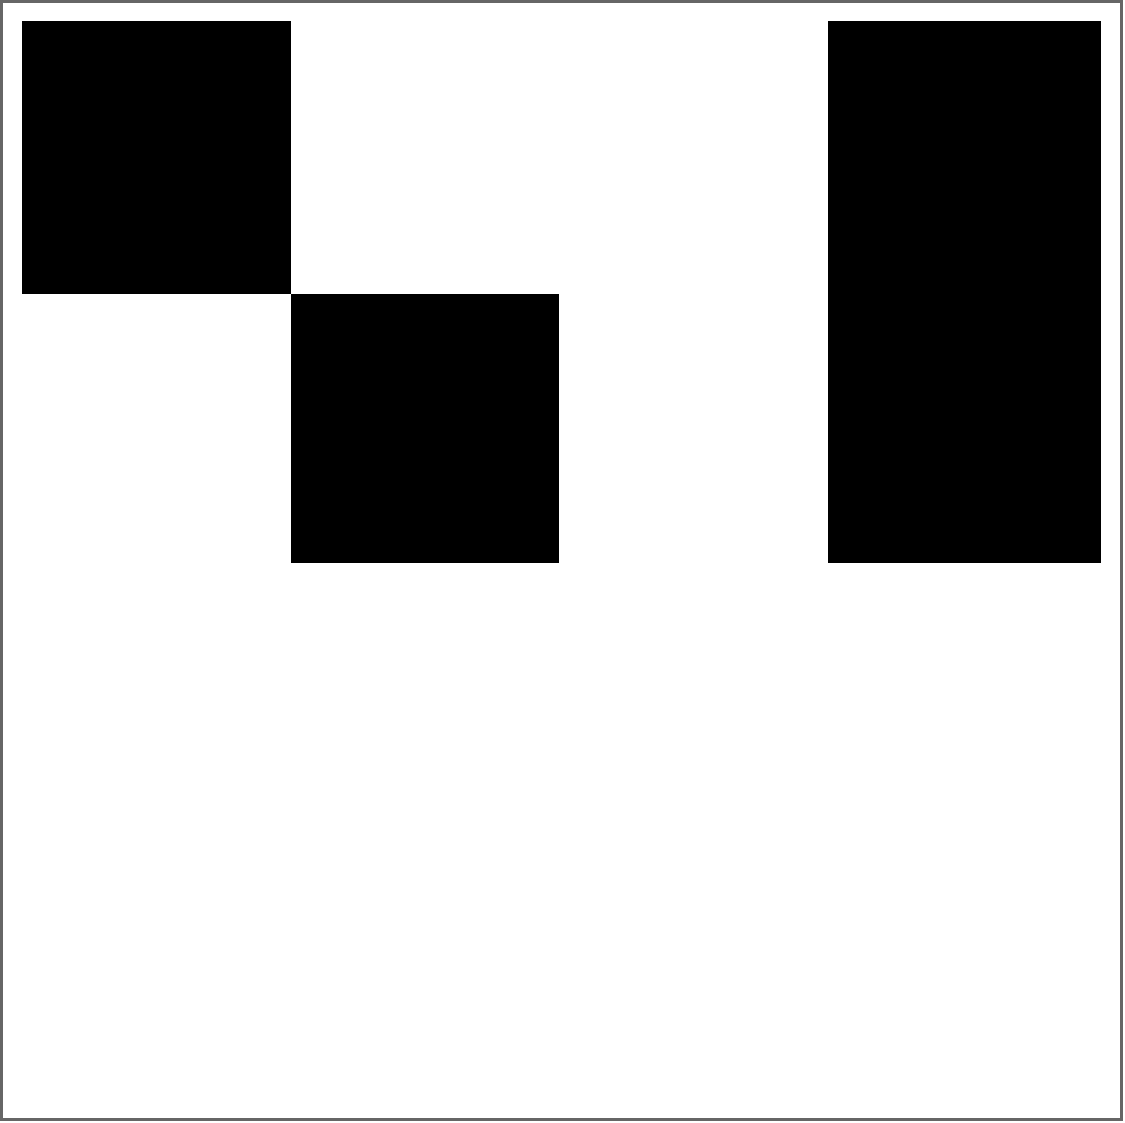
\includegraphics[width=3cm]{PCEoperation}
\caption{PCE operation that erases all Pauli components except 
for $r_{0,0}$, $r_{1,1}$, $r_{1,3}$, and $r_{0,3}$.}
\end{subfigure}
\begin{subfigure}{.5\textwidth}
\centering
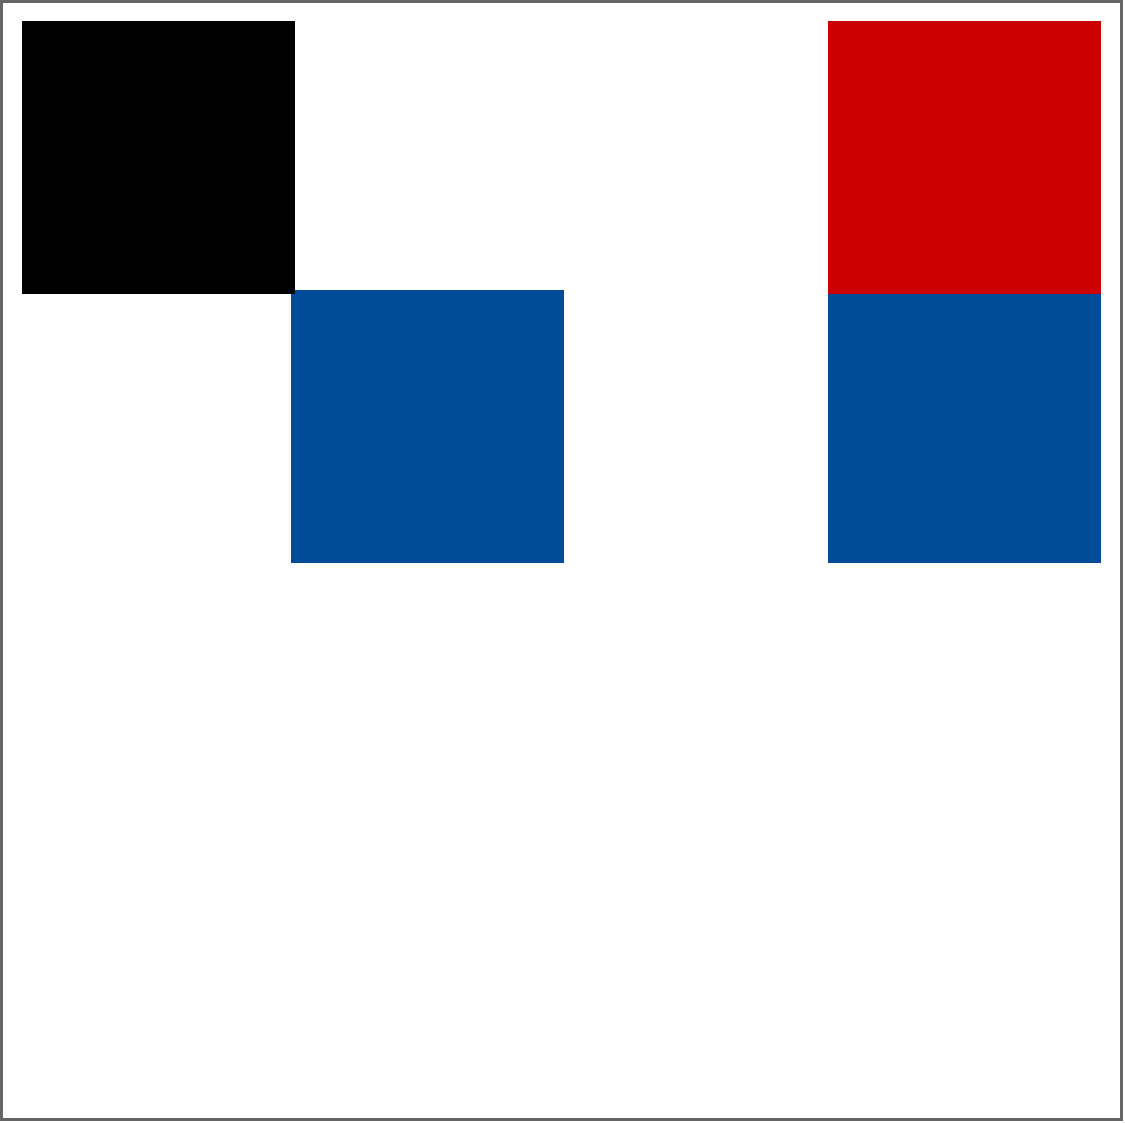
\includegraphics[width=3cm]{state}
\caption{Density matrix in Pauli basis with all components equal
to zero except for $r_{0,0}$, $r_{1,1}$, $r_{1,3}$, and $r_{0,3}$.}
\end{subfigure}
\end{figure}
% }}}

\subsection*{Hypothesis} % {{{
Let us denote $\PCE{n}$ the set of all PCE quantum channels for 
$n$ qubits.
\begin{conj}{}
There exists a set $\Gamma_n\subset\PCE{n}$ that is sufficient (and 
necessary?) to generate the rest of elements in $\PCE{n}$ as 
concatenations of different elements in $\Gamma_n$.
\end{conj}

Let us consider $\E_j\in\Gamma_n$ $(j=1,\ldots,4^{n}-1)$,
and $\Lambda\in\PCE{n}$. All $\Lambda$ are a composition of 
$\E_j$,
\begin{equation}\label{eq:PCE-characterization}
\underbrace{\E_{j_{2n}}\ldots\E_{j_1}}_{k\text{ elements}}=\Lambda,
\hspace{20pt}
j_l\neq j_{l+1},
\hspace{20pt}
k=1,\ldots,2n.
\end{equation}
% }}}
\subsection*{A way to find $\Gamma$} % {{{
PCE quantum channels in $\Gamma_n$ may be found as the quantum 
channels defined by the the coefficients $a_j^{\mu}$ of the $\tau_i$
in the eigenvalues expression of Choi matrix, with $a^{k}_{k}=0$ 
(instead of -1). Let us show the 2-qubits case as an example to illustrate this. 
The eigenvalues of Choi matrix of 2-qubits Pauli Channel are
\begin{align}
\lambda_{1}&=
 \tau _{0,0}+\tau _{0,1}-\tau _{0,2}-\tau _{0,3}+\tau _{1,0}+\tau _{1,1}-\tau _{1,2}-\tau
   _{1,3}-\tau _{2,0}-\tau _{2,1}+\tau _{2,2}+\tau _{2,3}-\tau _{3,0}-\tau _{3,1}+\tau
   _{3,2}+\tau _{3,3} \nonumber \\
\lambda_{2}&=   
 \tau _{0,0}-\tau _{0,1}-\tau _{0,2}+\tau _{0,3}+\tau _{1,0}-\tau _{1,1}-\tau _{1,2}+\tau
   _{1,3}-\tau _{2,0}+\tau _{2,1}+\tau _{2,2}-\tau _{2,3}-\tau _{3,0}+\tau _{3,1}+\tau
   _{3,2}-\tau _{3,3} \nonumber \\
\lambda_{3}&=
 \tau _{0,0}-\tau _{0,1}+\tau _{0,2}-\tau _{0,3}+\tau _{1,0}-\tau _{1,1}+\tau _{1,2}-\tau
   _{1,3}-\tau _{2,0}+\tau _{2,1}-\tau _{2,2}+\tau _{2,3}-\tau _{3,0}+\tau _{3,1}-\tau
   _{3,2}+\tau _{3,3} \nonumber \\
\lambda_{4}&=
 \tau _{0,0}+\tau _{0,1}+\tau _{0,2}+\tau _{0,3}+\tau _{1,0}+\tau _{1,1}+\tau _{1,2}+\tau
   _{1,3}-\tau _{2,0}-\tau _{2,1}-\tau _{2,2}-\tau _{2,3}-\tau _{3,0}-\tau _{3,1}-\tau
   _{3,2}-\tau _{3,3}\nonumber \\
\lambda_{5}&=
 \tau _{0,0}+\tau _{0,1}-\tau _{0,2}-\tau _{0,3}-\tau _{1,0}-\tau _{1,1}+\tau _{1,2}+\tau
   _{1,3}-\tau _{2,0}-\tau _{2,1}+\tau _{2,2}+\tau _{2,3}+\tau _{3,0}+\tau _{3,1}-\tau
   _{3,2}-\tau _{3,3}\nonumber \\
\lambda_{6}&=
 \tau _{0,0}-\tau _{0,1}-\tau _{0,2}+\tau _{0,3}-\tau _{1,0}+\tau _{1,1}+\tau _{1,2}-\tau
   _{1,3}-\tau _{2,0}+\tau _{2,1}+\tau _{2,2}-\tau _{2,3}+\tau _{3,0}-\tau _{3,1}-\tau
   _{3,2}+\tau _{3,3}\nonumber \\
\lambda_{7}&=
 \tau _{0,0}-\tau _{0,1}+\tau _{0,2}-\tau _{0,3}-\tau _{1,0}+\tau _{1,1}-\tau _{1,2}+\tau
   _{1,3}-\tau _{2,0}+\tau _{2,1}-\tau _{2,2}+\tau _{2,3}+\tau _{3,0}-\tau _{3,1}+\tau
   _{3,2}-\tau _{3,3}\nonumber \\
\lambda_{8}&=   
 \tau _{0,0}+\tau _{0,1}+\tau _{0,2}+\tau _{0,3}-\tau _{1,0}-\tau _{1,1}-\tau _{1,2}-\tau
   _{1,3}-\tau _{2,0}-\tau _{2,1}-\tau _{2,2}-\tau _{2,3}+\tau _{3,0}+\tau _{3,1}+\tau
   _{3,2}+\tau _{3,3}\nonumber \\
\lambda_{9}&=   
 \tau _{0,0}+\tau _{0,1}-\tau _{0,2}-\tau _{0,3}-\tau _{1,0}-\tau _{1,1}+\tau _{1,2}+\tau
   _{1,3}+\tau _{2,0}+\tau _{2,1}-\tau _{2,2}-\tau _{2,3}-\tau _{3,0}-\tau _{3,1}+\tau
   _{3,2}+\tau _{3,3}\nonumber \\
\lambda_{10}&=   
 \tau _{0,0}-\tau _{0,1}-\tau _{0,2}+\tau _{0,3}-\tau _{1,0}+\tau _{1,1}+\tau _{1,2}-\tau
   _{1,3}+\tau _{2,0}-\tau _{2,1}-\tau _{2,2}+\tau _{2,3}-\tau _{3,0}+\tau _{3,1}+\tau
   _{3,2}-\tau _{3,3}\nonumber \\
\lambda_{11}&=   
 \tau _{0,0}-\tau _{0,1}+\tau _{0,2}-\tau _{0,3}-\tau _{1,0}+\tau _{1,1}-\tau _{1,2}+\tau
   _{1,3}+\tau _{2,0}-\tau _{2,1}+\tau _{2,2}-\tau _{2,3}-\tau _{3,0}+\tau _{3,1}-\tau
   _{3,2}+\tau _{3,3}\nonumber \\
\lambda_{12}&=   
 \tau _{0,0}+\tau _{0,1}+\tau _{0,2}+\tau _{0,3}-\tau _{1,0}-\tau _{1,1}-\tau _{1,2}-\tau
   _{1,3}+\tau _{2,0}+\tau _{2,1}+\tau _{2,2}+\tau _{2,3}-\tau _{3,0}-\tau _{3,1}-\tau
   _{3,2}-\tau _{3,3}\nonumber \\
\lambda_{13}&=   
 \tau _{0,0}+\tau _{0,1}-\tau _{0,2}-\tau _{0,3}+\tau _{1,0}+\tau _{1,1}-\tau _{1,2}-\tau
   _{1,3}+\tau _{2,0}+\tau _{2,1}-\tau _{2,2}-\tau _{2,3}+\tau _{3,0}+\tau _{3,1}-\tau
   _{3,2}-\tau _{3,3}\nonumber \\
\lambda_{14}&=   
 \tau _{0,0}-\tau _{0,1}-\tau _{0,2}+\tau _{0,3}+\tau _{1,0}-\tau _{1,1}-\tau _{1,2}+\tau
   _{1,3}+\tau _{2,0}-\tau _{2,1}-\tau _{2,2}+\tau _{2,3}+\tau _{3,0}-\tau _{3,1}-\tau
   _{3,2}+\tau _{3,3}\nonumber \\
\lambda_{15}&=   
 \tau _{0,0}-\tau _{0,1}+\tau _{0,2}-\tau _{0,3}+\tau _{1,0}-\tau _{1,1}+\tau _{1,2}-\tau
   _{1,3}+\tau _{2,0}-\tau _{2,1}+\tau _{2,2}-\tau _{2,3}+\tau _{3,0}-\tau _{3,1}+\tau
   _{3,2}-\tau _{3,3}\nonumber \\
\lambda_{16}&=  
 \tau _{0,0}+\tau _{0,1}+\tau _{0,2}+\tau _{0,3}+\tau _{1,0}+\tau _{1,1}+\tau _{1,2}+\tau
   _{1,3}+\tau _{2,0}+\tau _{2,1}+\tau _{2,2}+\tau _{2,3}+\tau _{3,0}+\tau _{3,1}+\tau
   _{3,2}+\tau _{3,3}. 
\end{align}

Now, taking all $\tau_{i,j}$ with coefficients $-1$ equal to zero 
one is led to 16 elements of $\PCE{2}$ (one for each eigenvalue): \newline

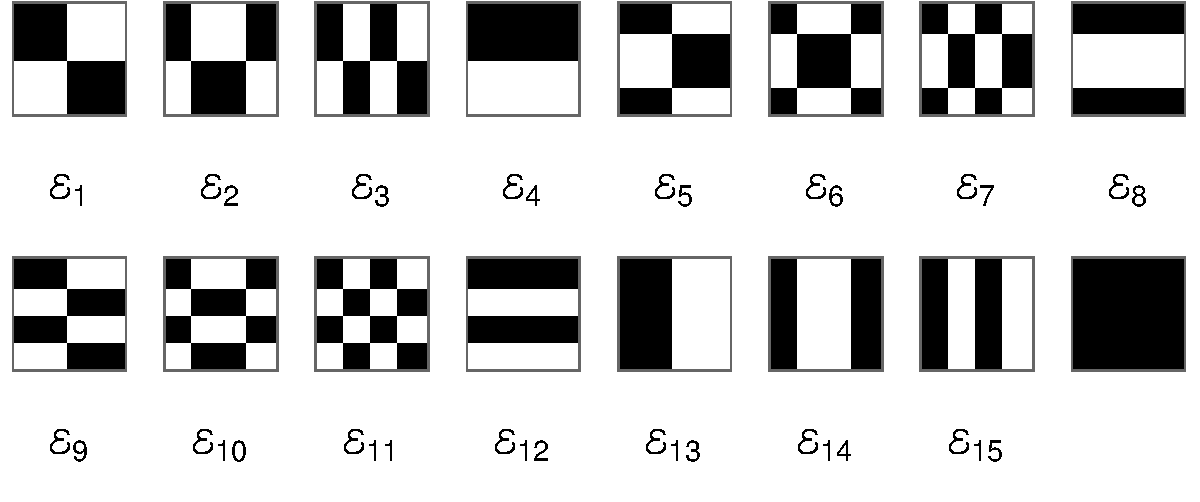
\includegraphics[width=\textwidth]{2Q-fundamentals}

The first 15 elements are the elements of $\Gamma_2$. 

For the sake
of completeness let us show how to construct all elements in $\PCE{2}$
from $\Gamma_2$. Recall that $\PCE{2}$ can be ordered in 
equivalence classes with PCE quantum channels that are 
connected via particle swaps and local permutations 
of basis.

\begin{itemize}
\item \textbf{8 components:} 
\begin{itemize}
\item C$_1^8$: $\E_{13}$\newline
\begin{tabular}{m{2cm} m{2cm} m{2cm}}
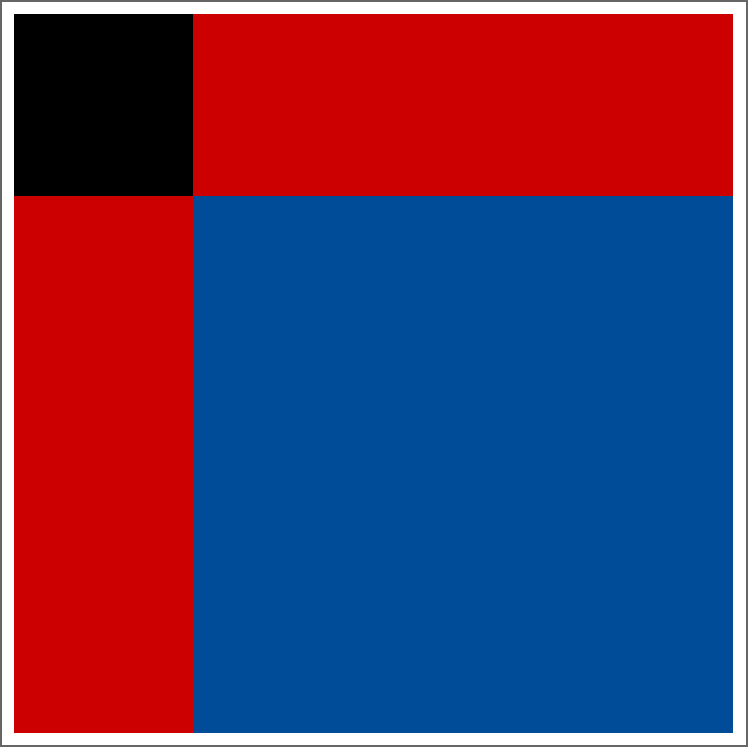
\includegraphics[width=2.2cm]{img-JA/id}  
& \hspace{0.8cm}$\longrightarrow$ 
& 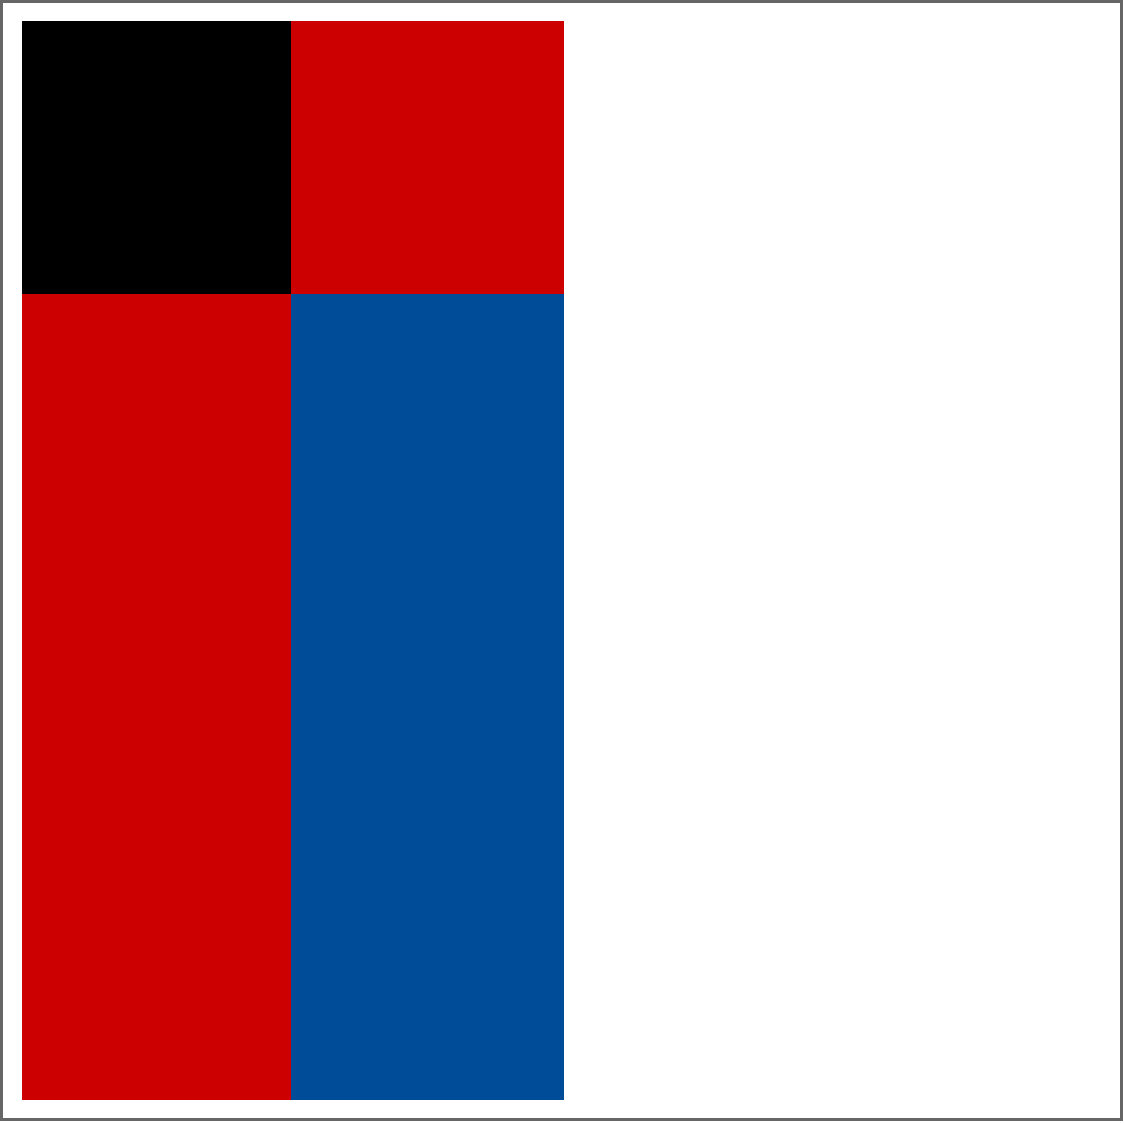
\includegraphics[width=2.2cm]{C81} \\ 
 & 
\includegraphics[width=2.2cm]{ruleC81} & 
\end{tabular} 

\item C$_2^8$: $\E_1$\newline
\begin{tabular}{m{2cm} m{2cm} m{2cm}}
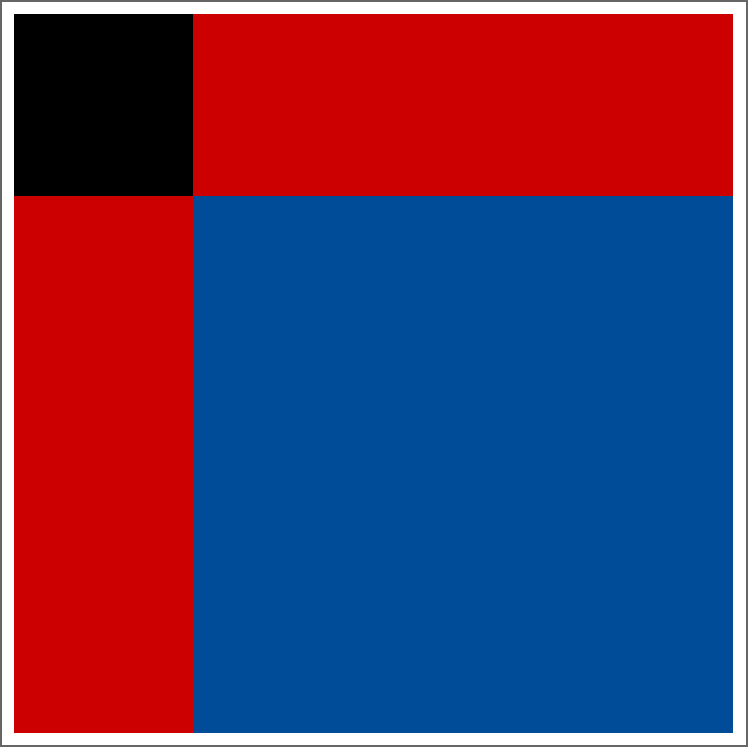
\includegraphics[width=2.2cm]{img-JA/id}  
& \hspace{0.8cm}$\longrightarrow$ 
& 
\includegraphics[width=2.2cm]{img-JA/8comp}\\ 
 & 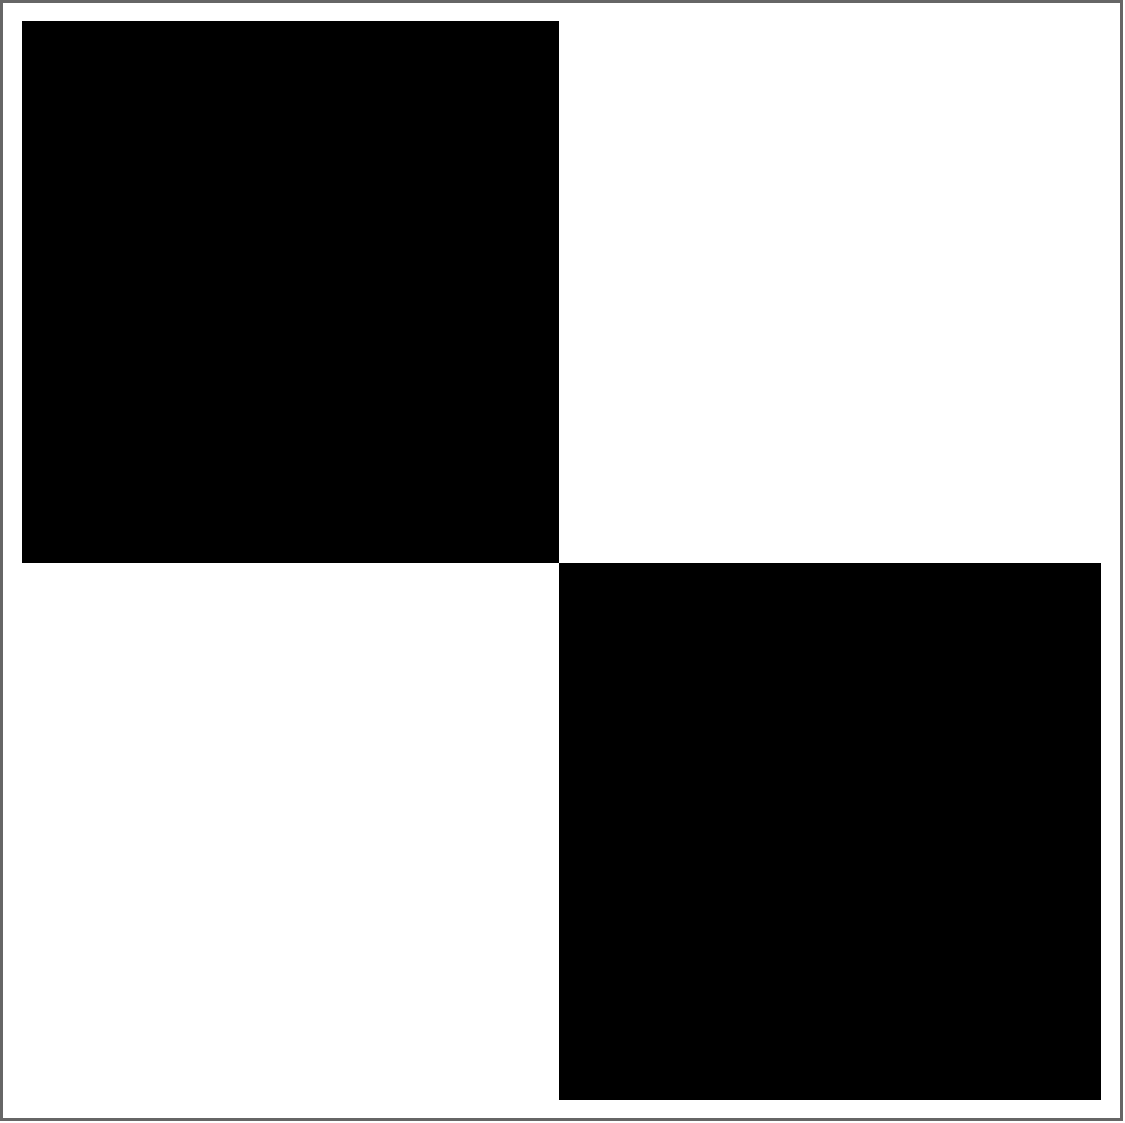
\includegraphics[width=2.2cm]{img-JA/16To8} &  
\end{tabular} 
\end{itemize}

\item \textbf{4 components:} \newline
\begin{itemize}
\item C$_1^4$: $\E_{15}\E_{13}$\newline
\begin{tabular}{m{2cm} m{2cm} m{2cm} m{2cm} m{2cm}}
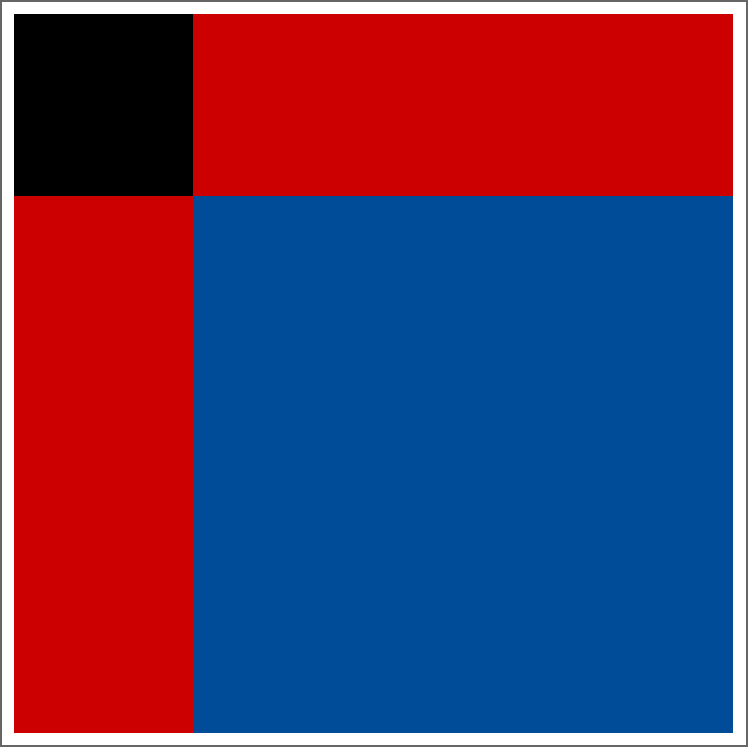
\includegraphics[width=2.2cm]{img-JA/id}  
& \hspace{0.8cm}$\longrightarrow$ 
& 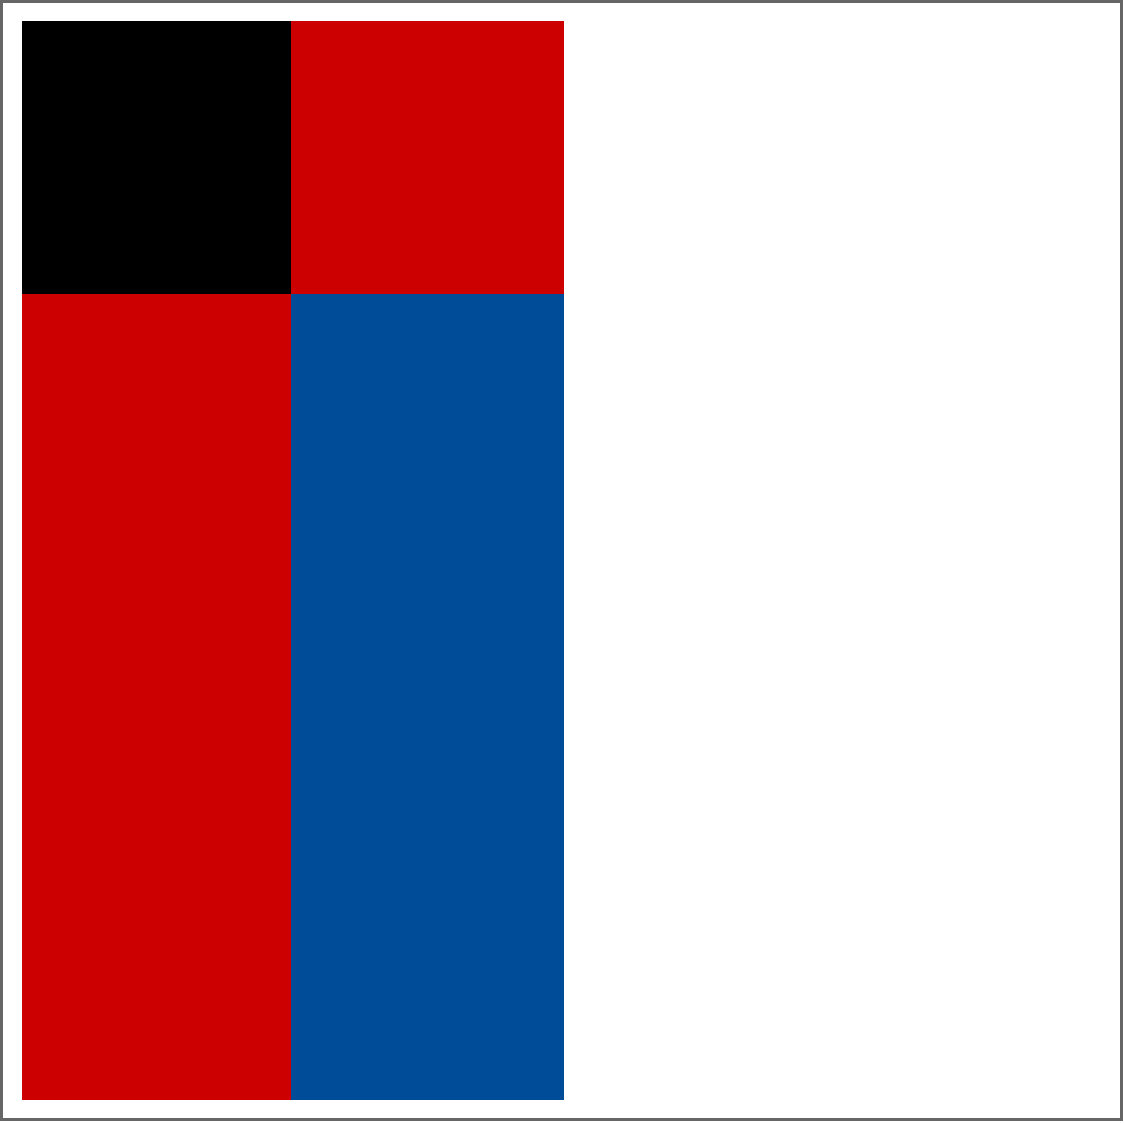
\includegraphics[width=2.2cm]{C81} 
& \hspace{0.8cm}$\longrightarrow$ 
& 
\includegraphics[width=2.2cm]{C41}\\ 
 & 
\includegraphics[width=2.2cm]{ruleC81} &  
 & 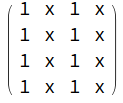
\includegraphics[width=2.2cm]{ruleC81_2} &\\ 
\end{tabular} 

\item C$_2^4$: $\E_{13}\E_1$\newline
\begin{tabular}{m{2cm} m{2cm} m{2cm} m{2cm} m{2cm}}
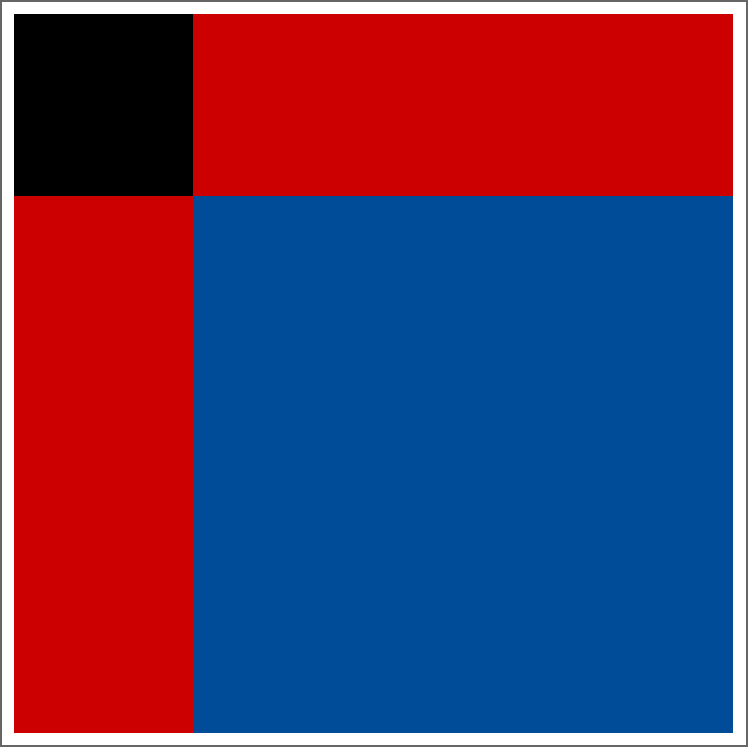
\includegraphics[width=2.2cm]{img-JA/id}  
& \hspace{0.8cm}$\longrightarrow$ 
& 
\includegraphics[width=2.2cm]{img-JA/8comp} 
& \hspace{0.8cm}$\longrightarrow$ 
& 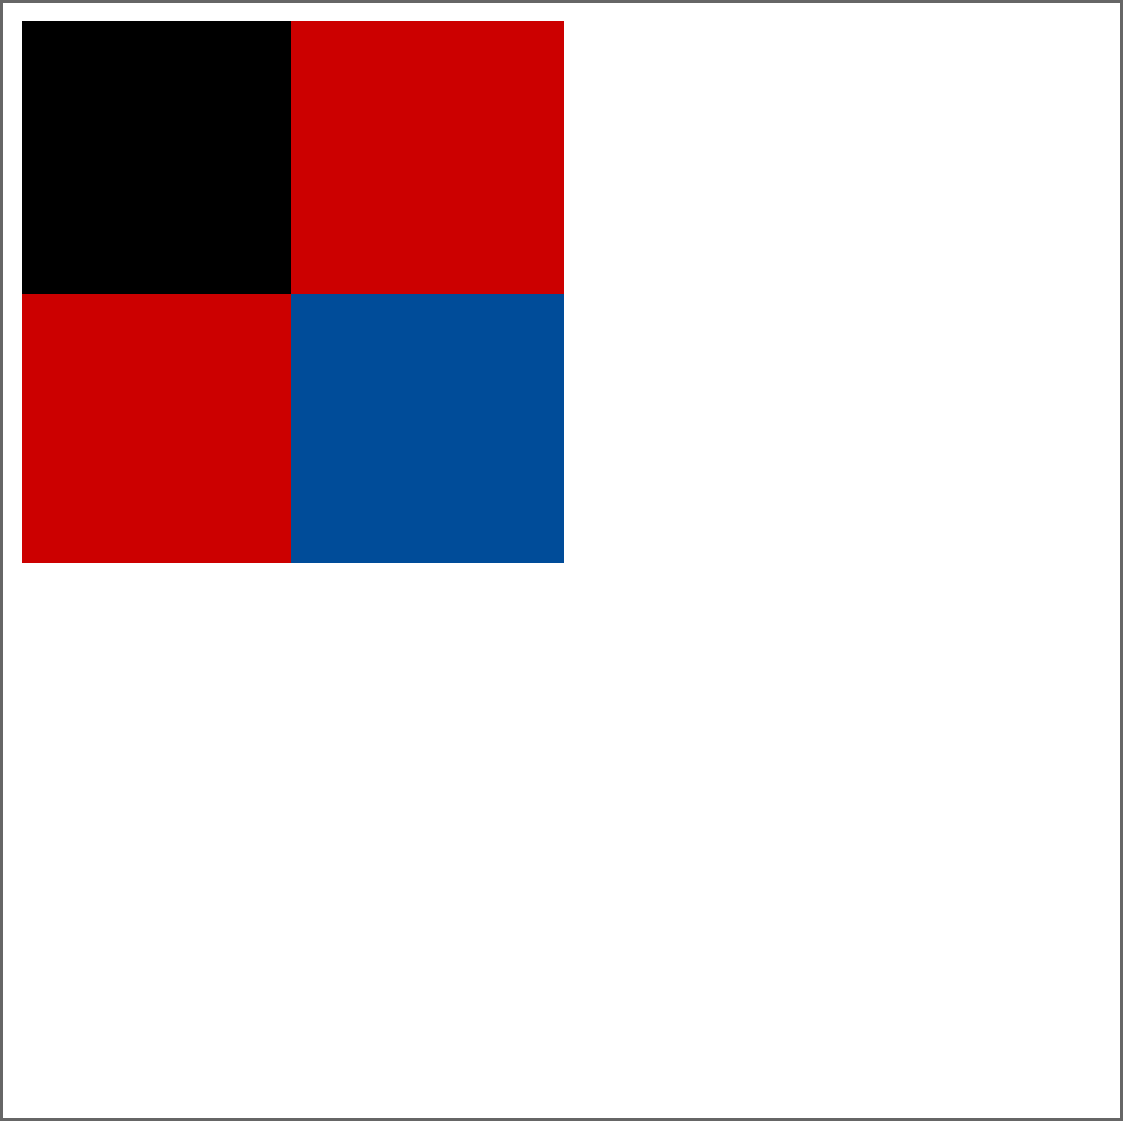
\includegraphics[width=2.2cm]{C42}\\ 
 & 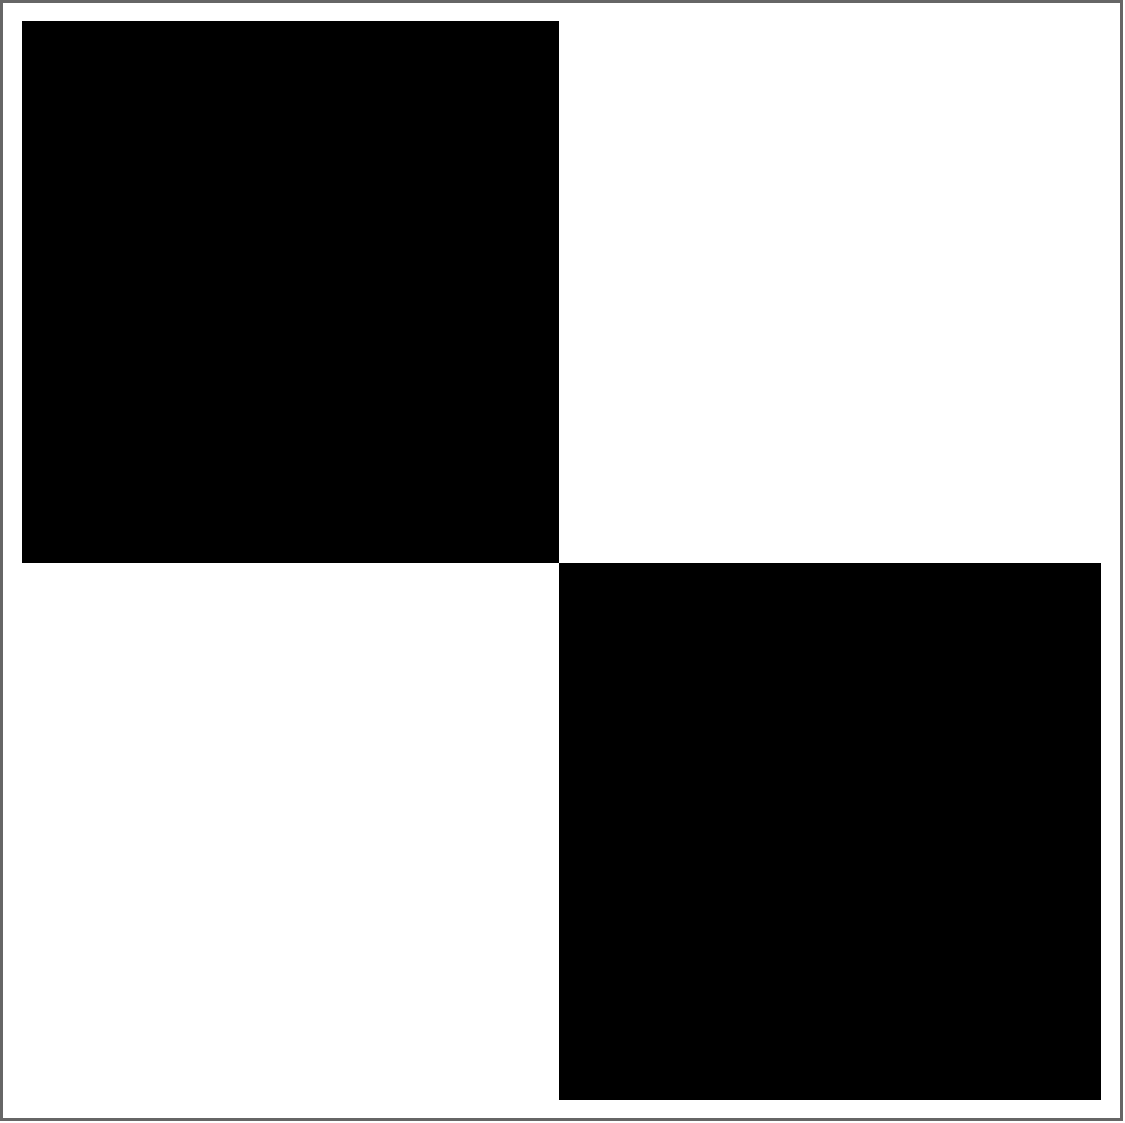
\includegraphics[width=2.2cm]{img-JA/16To8} &  
 & 
\includegraphics[width=2.2cm]{ruleC81} &\\ 
\end{tabular} 

\pagebreak
\item C$_3^4$: $\E_{15}\E_{1}$\newline
\begin{tabular}{m{2cm} m{2cm} m{2cm} m{2cm} m{2cm}}
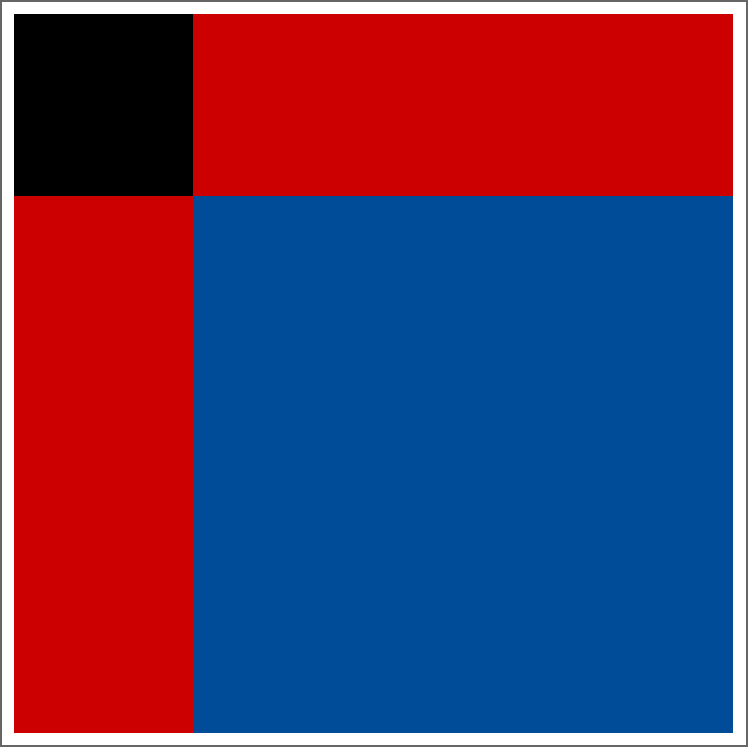
\includegraphics[width=2.2cm]{img-JA/id}  
& \hspace{0.8cm}$\longrightarrow$ 
& 
\includegraphics[width=2.2cm]{img-JA/8comp} 
& \hspace{0.8cm}$\longrightarrow$ 
& 
\includegraphics[width=2.2cm]{C43}\\ 
 & 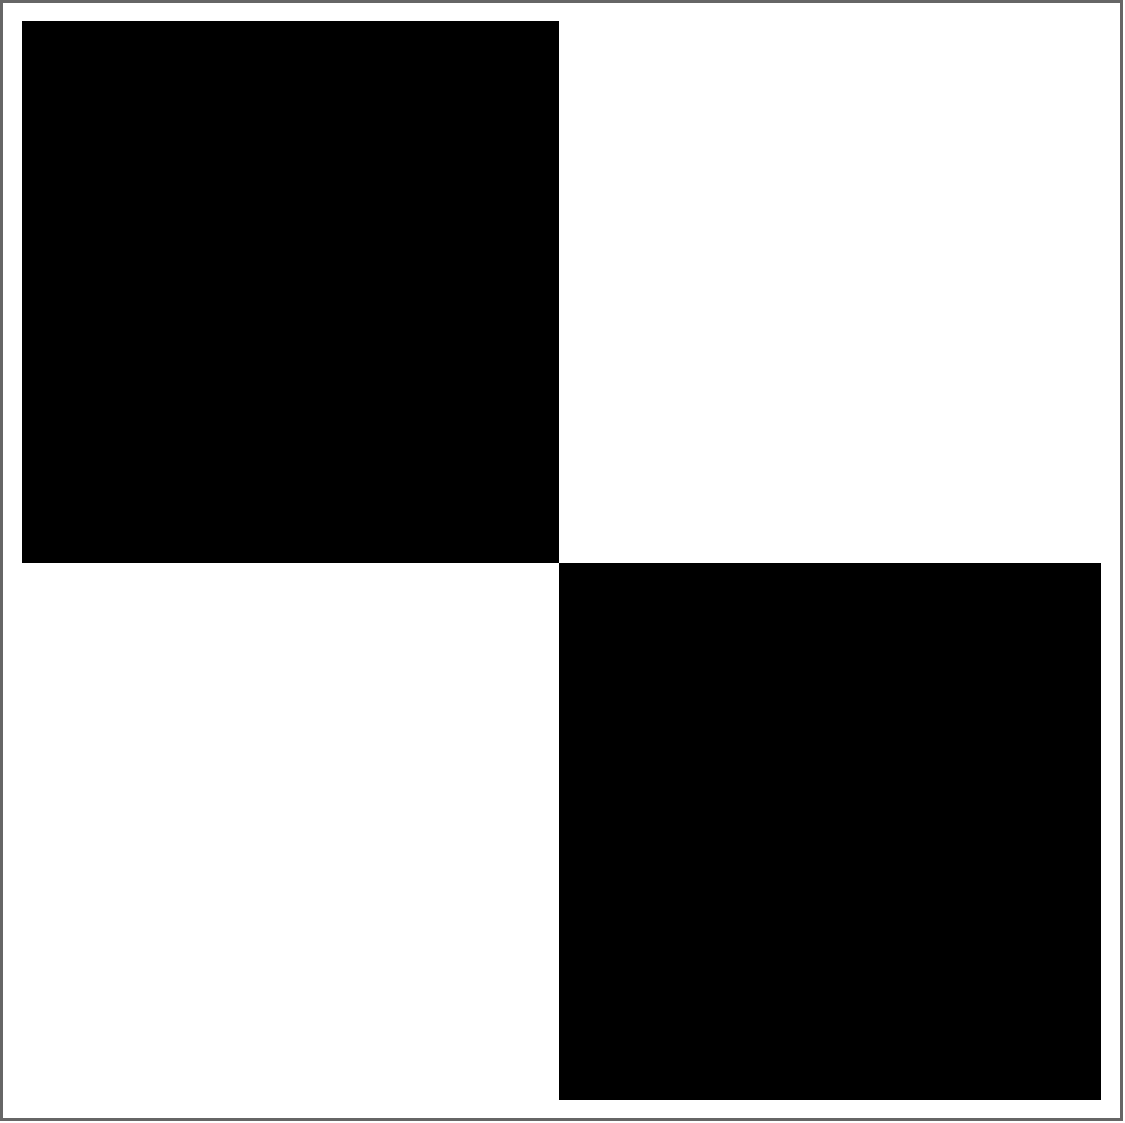
\includegraphics[width=2.2cm]{img-JA/16To8} &  
 & 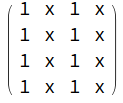
\includegraphics[width=2.2cm]{ruleC81_2} &\\ 
\end{tabular} 

\item C$_4^4$: $\E_7\E_1$\newline
\begin{tabular}{m{2cm} m{2cm} m{2cm} m{2cm} m{2cm}}
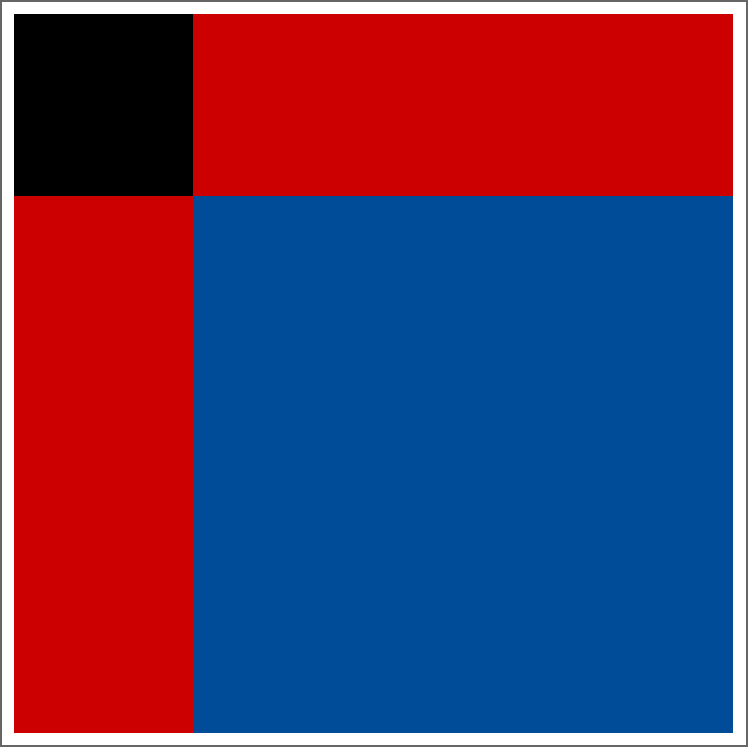
\includegraphics[width=2.2cm]{img-JA/id}  
& \hspace{0.8cm}$\longrightarrow$ 
& 
\includegraphics[width=2.2cm]{img-JA/8comp} 
& \hspace{0.8cm}$\longrightarrow$ 
& 
\includegraphics[width=2.2cm]{img-JA/4comp}\\ 
 & 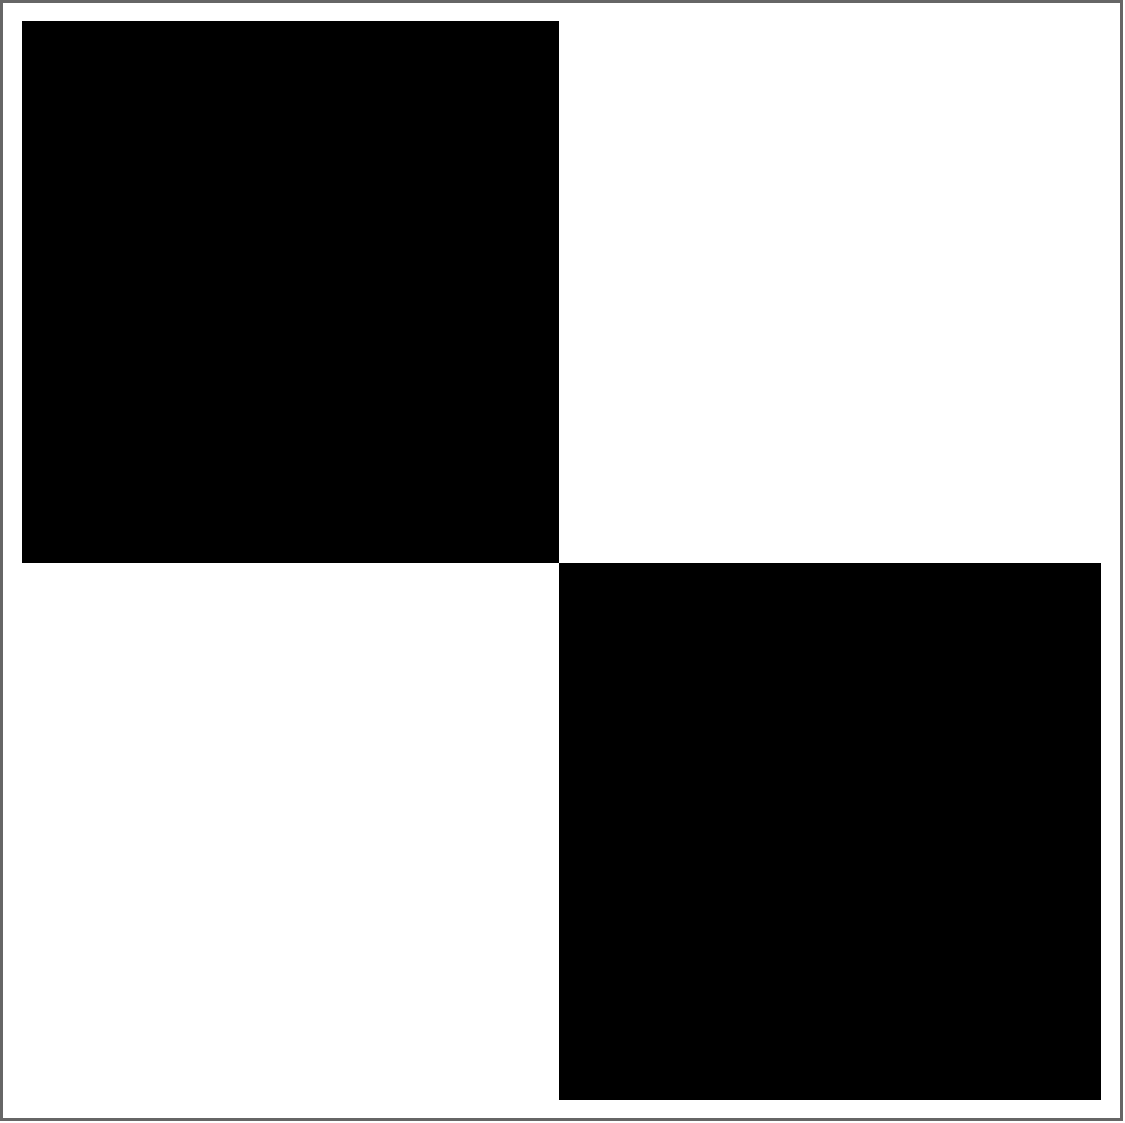
\includegraphics[width=2.2cm]{img-JA/16To8} &  
 & 
\includegraphics[width=2.2cm]{img-JA/8To4} &\\ 
\end{tabular} 
\end{itemize}


\item \textbf{2 components:}\newline
\begin{itemize}
\item C$_1^2$: $\E_{15}\E_{14}\E_1$\newline
\begin{tabular}{m{2cm} m{2cm} m{2cm} m{2cm} m{2cm} m{2cm} m{2cm}}
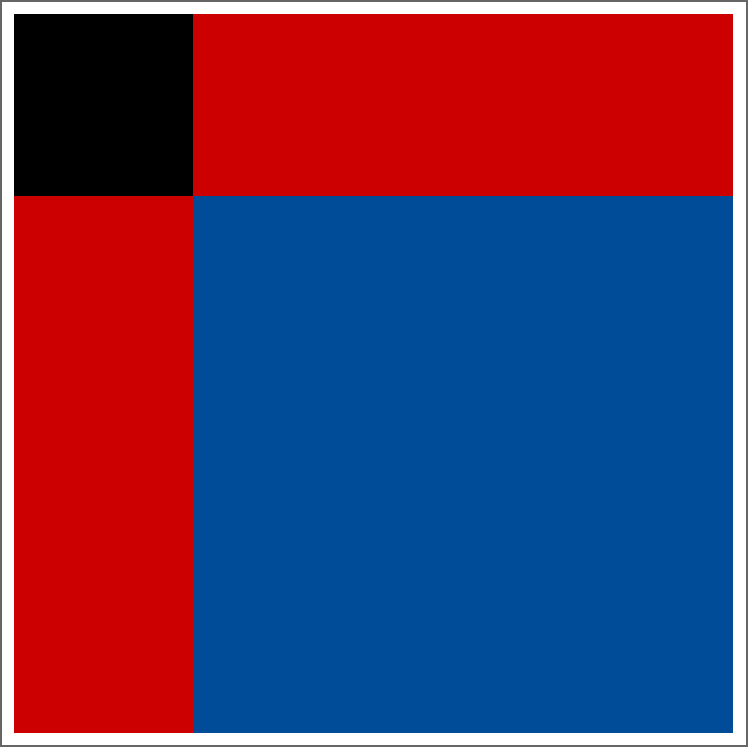
\includegraphics[width=2.2cm]{img-JA/id}  
& \hspace{0.8cm}$\longrightarrow$ 
& 
\includegraphics[width=2.2cm]{img-JA/8comp} 
& \hspace{0.8cm}$\longrightarrow$ 
& 
\includegraphics[width=2.2cm]{C43}
& \hspace{0.8cm}$\longrightarrow$ 
& 
\includegraphics[width=2.2cm]{C21}\\ 
 & 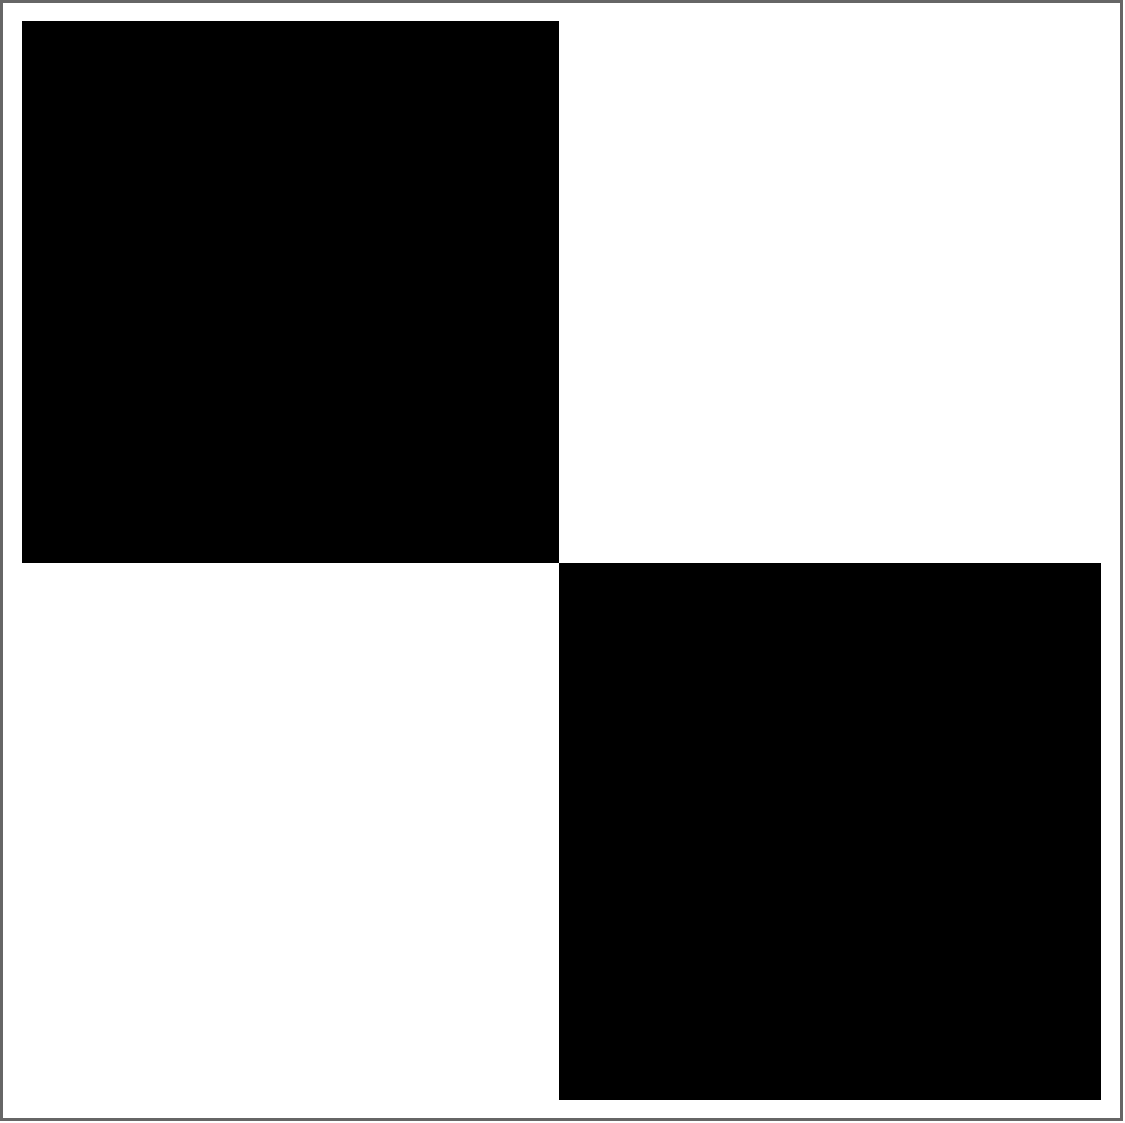
\includegraphics[width=2.2cm]{img-JA/16To8} &  
 & 
\includegraphics[width=2.2cm]{semefue} &
 & 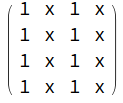
\includegraphics[width=2.2cm]{ruleC81_2} &\\ 
\end{tabular} 

\item C$_2^2$: $\E_6\E_7\E_1$\newline
\begin{tabular}{m{2cm} m{2cm} m{2cm} m{2cm} m{2cm} m{2cm} m{2cm}}
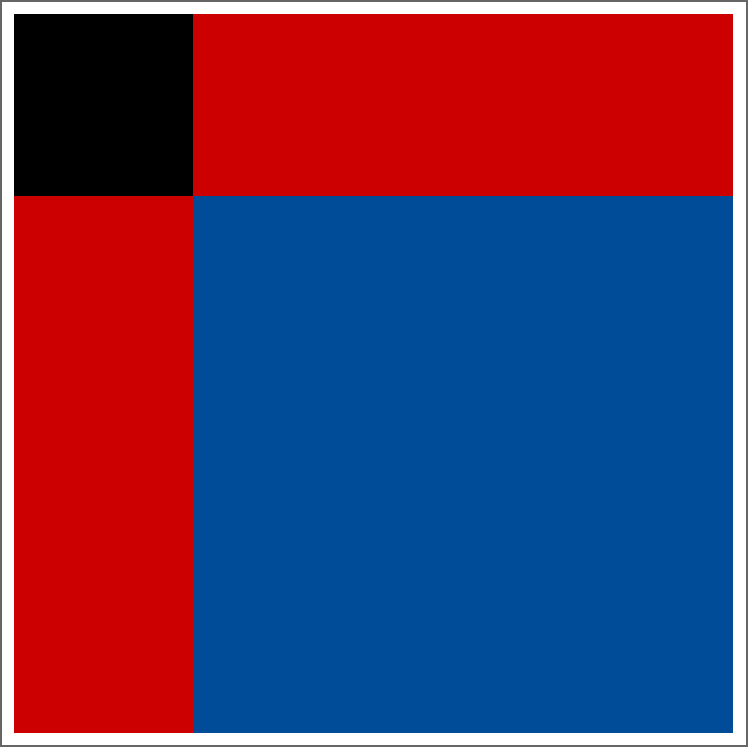
\includegraphics[width=2.2cm]{img-JA/id}  
& \hspace{0.8cm}$\longrightarrow$ 
& 
\includegraphics[width=2.2cm]{img-JA/8comp} 
& \hspace{0.8cm}$\longrightarrow$ 
& 
\includegraphics[width=2.2cm]{img-JA/4comp}
& \hspace{0.8cm}$\longrightarrow$ 
& 
\includegraphics[width=2.2cm]{C22}\\ 
 & 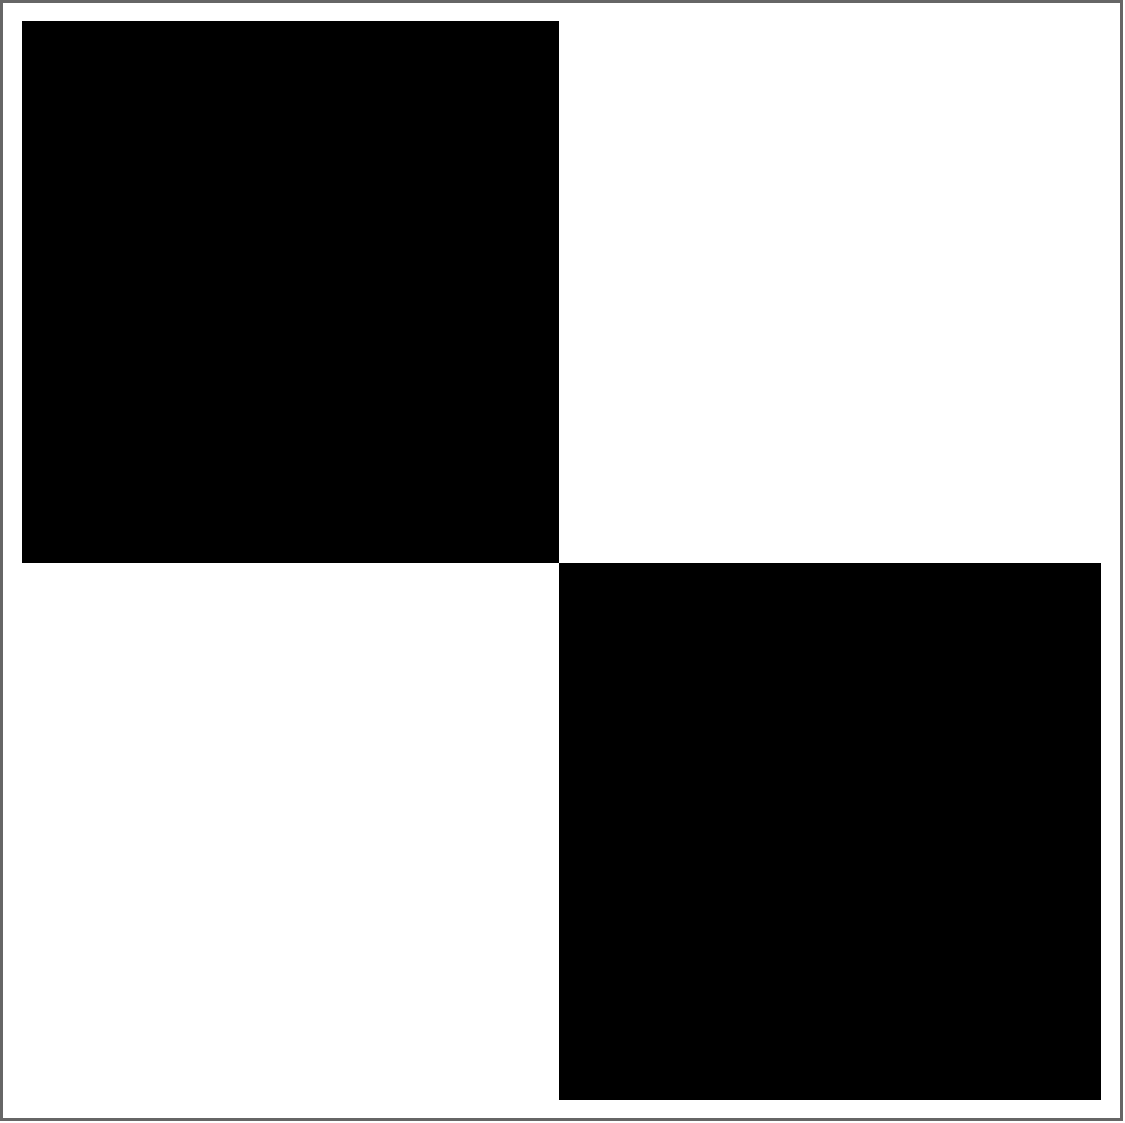
\includegraphics[width=2.2cm]{img-JA/16To8} &  
 & 
\includegraphics[width=2.2cm]{img-JA/8To4} &
 & 
\includegraphics[width=2.2cm]{otroTambien}\\ 
\end{tabular}
\end{itemize}


\pagebreak
\item \textbf{1 component:} $\E_9\E_6\E_7\E_1$\newline
\begin{tabular}{m{2cm} m{2cm} m{2cm}}

\includegraphics[width=2.2cm]{C22}
& \hspace{0.8cm}$\longrightarrow$ 
& 
\includegraphics[width=2.2cm]{depolarizing} \\ 
 & 
\includegraphics[width=2.2cm]{img-JA/otro} &  \\ 
\end{tabular}
\end{itemize}

\begin{conj}
Only $n$ elements in $\Gamma_n$ are sufficient to generate the 
remaining elements.
\end{conj}
% }}}
\subsection{Numerical Results} % {{{
Hypothesis 1 has strong numerical support. The search for PCE quantum
channels has been done in two different ways:
\begin{enumerate}
\item Using the inequalities in \eqref{eq:inequalities-PCE} to test CP of 
all PCE operations (even the ones that do not follow the power-of-2 rule).
\item Using hypoteshis 1.
\end{enumerate}
Both methods have analyzed the cases of 1, 2, 3 and partially 4 qubits. 
Both of them get the same results. 

\begin{figure}[H]
  \centering
  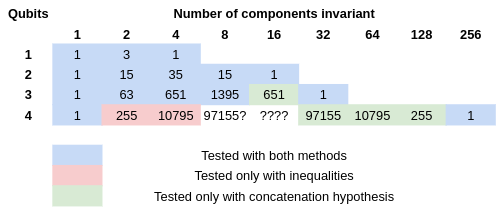
\includegraphics[width=.6\textwidth]{cuadro}
\end{figure}
% }}}
% }}}
\section{Things to do and questions to answer} % {{{
\begin{enumerate}
\item This characterization may explain the power-of-2 rule. 
It is quite obvious (in the figures representation) that the concatenation
always erases half of the number of non-zero components. A proof 
for that is missing.
\item Analytic proof for \eqref{eq:inequalities-PCE}. 
\item Analytic proof that \eqref{eq:PCE-characterization} is necessary 
and sufficient to find all elements in $\PCE{n}$.
\item Analytic proof that taking $-1\to 0$ for $a_k^k$ leads to CP.
I suggest using particle swaps and local basis permutation in order 
to reduce the problem to $n$ inequalities.
\item Find a way to count PCE channels.
\end{enumerate}
% }}}

\section{Progress}
\subsection{An idea to prove equation \eqref{eq:eigvals-PCE}}
A density matrix of 1 qubit in Pauli matrices basis is written as
\begin{align}
\rho=\frac{1}{2}\sum_{i=0}^3r_i\sigma_i,
\end{align}
where $\sigma_i$ are a $2\times2$ identity plus Pauli matrices.
For 2 qubits, in the general case, the density matrix cannot be written as
\begin{align}\label{eq:2qubits-densityM-PauliBasis-separable}
\rho&=\frac{1}{4}\qty(\sum_{i=0}^3r_i\sigma_i
\ot
\sum_{j=0}^3r_j\sigma_j)
\end{align}
because a 2-qubits state is not separable, in general. Therefore, 
the density matrix is written as
\begin{align}
\rho=\frac{1}{4}\sum_{i,j=0}^3r_{i,j}\sigma_{i,j}.
\end{align}
In some sense, expanding 
\eqref{eq:2qubits-densityM-PauliBasis-separable}
\begin{align}
\frac{1}{4}\qty(\sum_{i=0}^3r_i\sigma_i
\ot
\sum_{j=0}^3r_j\sigma_j)
&=\frac{1}{4}\qty(
\1_{4}\ot\1_{4}+\1\ot\sum_{j=1}^3r_j\sigma_j+
\sum_{i=1}^3r_i\sigma_i\ot\1+
\sum_{i=1}^3r_i\sigma_i\ot\sum_{j=1}^3r_j\sigma_j
)
\end{align}
makes us a hint realize that, in the general case, the components
of 2-qubits density matrix in tensor products of Pauli matrices basis are
\begin{align}
r_ir_j&\to r_{i.j},&\ r_i&\to r_{i,0},&\ r_j &\to r_{0,j}.
\end{align}
It follows that $n$-quits density matrix is
\begin{align}
\rho=\frac{1}{2^n}\sum_{j_1,\ldots,j_n=0}^3
r_{j_1,\ldots,j_n}\sigma_{j_1}\ot\ldots\ot\sigma_{j_n},
\end{align}
therefore,
\begin{align}
\label{eq:general-comp-of-density-matrix-in-Pauli-matrices-basis}
r_{j_1}\ldots r_{j_k}\ldots r_{j_n}&\to r_{j_1,\ldots,j_n}, &
r_{j_k}&\to r_{0,\ldots,j_k,\ldots,0},
\end{align}
where 
\begin{align}
r_{j_1}\ldots r_{j_k}\ldots r_{j_n}&\neq r_{j_1,\ldots,j_n}, &
r_{j_k}&\neq r_{0,\ldots,j_k,\ldots,0},
\end{align}

Now, the state $\rho_{\E}$ isomorphic to the Choi matrix $D_{\E}$
(is this written ok?) of a 1-qubit PCE channel~$\E$~is
\begin{align}
\rho_{\E}&=\sum_{i=0}^3\lambda_i \dyad{\sigma_i}{\sigma_i},
\end{align}
where $\ket{\sigma_i}$ are the vectorized $\sigma_i$ and
$\lambda_i$ are (this has been shown analytically)
\begin{align}\label{eq:eigvals-1q-choi}
\lambda_0&=\frac{1}{4}\qty(1+\tau_1+\tau_2+\tau_3), &
\lambda_1&=\frac{1}{4}\qty(1+\tau_1-\tau_2-\tau_3),\nonumber\\
\lambda_2&=\frac{1}{4}\qty(1-\tau_1+\tau_2-\tau_3), &
\lambda_3&=\frac{1}{4}\qty(1-\tau_1-\tau_2+\tau_3).
\end{align}

I claim that, in the same sense of 
\eqref{eq:general-comp-of-density-matrix-in-Pauli-matrices-basis},
the eigenvalues of $\rho_{\E}$ of $n$-qubits PCE quantum channel
$\E$ are of the form
\begin{align}
\lambda_{j_1}\ldots \lambda_{j_k}\ldots \lambda_{j_n}
&\to\lambda_{j_1,\ldots,j_n}, &
\lambda_{j_k}&\to\lambda_{0,\ldots,j_k,\ldots,0},
\end{align}
where $\lambda_k$ are the eigenvalues \eqref{eq:eigvals-1q-choi}.

\section{Number of PCE channels by the ratio of components 
left invariant}
\begin{itemize}
\item 1$/$2 of total components invariant:
\begin{align}
4^n-1
\end{align}

\item 1$/$4 of total components invariant:
\begin{align}
\frac{\binom{4^n-1}{2}}{3},
\end{align}

\item 1$/$8 of total components invariant:
\begin{align}
\frac{\binom{4^n-1}{3}-\binom{4^n-1}{2}/3}{28}
\end{align}

\item 1$/$16 of total components invariant:
\begin{align}
\frac{\binom{4^n-1}{4}-35\qty(\frac{\binom{4^n-1}{3}-\binom{4^n-1}{2}/3}{28})}{840}
\end{align}
\end{itemize}

\begin{table}[h!]
\tiny
\begin{tabular}{llllccccccclll}
{\color[HTML]{FF0000} \textbf{1}} &                       &                           &                                & \multicolumn{1}{l}{} & \multicolumn{1}{l}{}               & \cellcolor[HTML]{FCE5CD}\textbf{1}   & \textbf{3}                             & \textbf{1}                              & \multicolumn{1}{l}{}                    & \multicolumn{1}{l}{}                &                                                       &                                    &                                \\
{\color[HTML]{FF0000} \textbf{2}} &                       &                           &                                & \multicolumn{1}{l}{} & \cellcolor[HTML]{FCE5CD}\textbf{1} & \cellcolor[HTML]{CFE2F3}\textbf{15}  & \cellcolor[HTML]{FCE5CD}\textbf{35}    & \textbf{15}                             & \textbf{1}                              & \multicolumn{1}{l}{}                &                                                       &                                    &                                \\
{\color[HTML]{FF0000} \textbf{3}} &                       &                           &                                & \textbf{1}           & \textbf{63}                        & \cellcolor[HTML]{FCE5CD}\textbf{651} & \cellcolor[HTML]{CFE2F3}\textbf{1,395} & \cellcolor[HTML]{FCE5CD}\textbf{651}    & \textbf{63}                             & \textbf{1}                          &                                                       &                                    &                                \\
{\color[HTML]{FF0000} \textbf{4}} &                       &                           & \multicolumn{1}{c}{\textbf{1}} & \textbf{255}         & \textbf{10,795}                    & 97,155                               & \cellcolor[HTML]{FCE5CD}200,787        & \cellcolor[HTML]{CFE2F3}\textbf{97,155} & \cellcolor[HTML]{FCE5CD}\textbf{10,795} & \textbf{255}                        & \multicolumn{1}{c}{\textbf{1}}                        &                                    &                                \\
{\color[HTML]{FF0000} \textbf{5}} &                       & \multicolumn{1}{c}{1}     & \multicolumn{1}{c}{1,023}      & 174,251              & 6,347,715                          & 53,743,987                           & \multicolumn{1}{l}{}                   & \cellcolor[HTML]{FCE5CD}53,743,987      & \cellcolor[HTML]{CFE2F3}6,347,715       & \cellcolor[HTML]{FCE5CD}174,251     & \multicolumn{1}{c}{\textbf{1,023}}                    & \multicolumn{1}{c}{\textbf{1}}     &                                \\
{\color[HTML]{FF0000} \textbf{6}} & \multicolumn{1}{c}{1} & \multicolumn{1}{c}{4,095} & \multicolumn{1}{c}{2,794,155}  & 408,345,795          & 13,910,980,083                     & \multicolumn{1}{l}{}                 & \multicolumn{1}{l}{}                   & \multicolumn{1}{l}{}                    & \cellcolor[HTML]{FCE5CD}13,910,980,083  & \cellcolor[HTML]{CFE2F3}408,345,795 & \multicolumn{1}{c}{\cellcolor[HTML]{FCE5CD}2,794,155} & \multicolumn{1}{c}{\textbf{4,095}} & \multicolumn{1}{c}{\textbf{1}}
\end{tabular}
\end{table}
\section*{David's ideas}
\section{Alejo's ideas}
% 
\subsection{Eigenvalues of the Choi matrix}
% 
Due to the fact that the Pauli matrices and the identity form a basis of the Hilber-Shmidt space, the state of a qubit may be written as
% 
\begin{equation}
 \hat{\rho}=\frac{1}{2}\sum_{j,k=0}^1r_{jk}\hat{v}_{jk},
\end{equation}
%
where $\hat{v}_{00}=\dsone$, $\hat{v}_{01}=\hat{\sigma}_x$, $\hat{v}_{10}=i\hat{\sigma}_y$ and $\hat{v}_{11}=\hat{\sigma}_z$.
% 
Rewriting $\hat{\rho}$ in ``vector" notation, we have
%
\begin{equation}
 \vec{\rho}=\frac{1}{2}\sum_{jk=0}^1r_{jk}\vec{v}_{jk},
\end{equation}
%
The action of a quantum operation $\hat{M}$ (in its matrix form), capable of modifying each one of the coefficients $r_{jk}$ independently may be written as
%
\begin{equation}
 \hat{M}\vec{\rho}=\frac{1}{2}\sum_{jk=0}^1\tau_{jk}r_{jk}\vec{v}_{jk}.
\end{equation}
%
In our particular case (PCE operations), $\tau_{jk}=\{0,1\}$. 

In order to determine whether any specific operation, characterized by the set of coefficients $\{\tau_{jk}\}$ corresponds to a quantum channel, we must ensure that the eigenvalues associated to the Choi matrix are non-negative. For this, let write $\hat{M}$ in the vector Pauli basis
%
\begin{equation}
 \hat{M}=\sum_{jk=0}^1\tau_{jk}~\vec{v}_{jk}\vec{v}_{jk}^\intercal.
 \label{EQA1}
\end{equation}
%
On the other hand, it is easy to show that the elements of the computational and Pauli bases are related by $\vec{u}=\hat{T}\vec{v}$
\begin{equation}
\vec{u}=\begin{pmatrix}
\hat{u}_{00} \\ \hat{u}_{01} \\ \hat{u}_{10} \\ \hat{u}_{11}
\end{pmatrix}=\frac{1}{2}\begin{pmatrix}
1 & 0 & 0 & 1\\
0 & 1 & 1 & 0\\
0 & 1 & -1 & 0\\
1 & 0 & 0 & -1
\end{pmatrix} \begin{pmatrix}
\hat{v}_{00} \\ \hat{v}_{01} \\ \hat{v}_{10} \\ \hat{v}_{11}
\end{pmatrix},
\end{equation}
% 
where $\hat{u}_{jk}=\dyad{j}{k}$. The inverse relation reads $\vec{v}=\hat{S}\vec{u}$
\begin{equation}
\vec{v}=\begin{pmatrix}
\hat{v}_{00} \\ \hat{v}_{01} \\ \hat{v}_{10} \\ \hat{v}_{11}
\end{pmatrix}=\begin{pmatrix}
1 & 0 & 0 & 1\\
0 & 1 & 1 & 0\\
0 & 1 & -1 & 0\\
1 & 0 & 0 & -1
\end{pmatrix} \begin{pmatrix}
\hat{u}_{00} \\ \hat{u}_{01} \\ \hat{u}_{10} \\ \hat{u}_{11}
\end{pmatrix}.
\end{equation}
% 
Thus, for this ``indexing choice" of the elements of the bases, the transformation matrices satisfy $\hat{S}=2\hat{T}$. Then one can relate the bases elements in a compact form as
% 
\begin{equation}
 \vec{v}_{jk}=\sum_{mn=0}^1S_{mn}^{(jk)}\vec{u}_{mn},
\end{equation}
% 
by substituting this in Eq. \ref{EQA1} we get $\hat{M}$ in the computational basis
% 
\begin{align}
 \hat{M}=&\sum_{jk=0}^1\tau_{jk}~\left(\sum_{mn=0}^1S_{mn}^{(jk)}\vec{u}_{mn} \right) \left(\sum_{pq=0}^1S_{jk}^{(pq)}\vec{u}^\intercal_{pq} \right),\\
 =&\sum_{mnpq=0}^1\left(\sum_{jk=0}^1 S_{mn}^{(jk)}S_{jk}^{(pq)}  \tau_{jk} \right) \vec{u}_{mn}\vec{u}^\intercal_{pq}.\\
 &\sum_{mnpq=0}^1 M_{\substack{mn\\pq}} ~\vec{u}_{mn}\vec{u}^\intercal_{pq}.
\end{align}
% 
In order to obtain the Choi matrix $\hat{M}^c$, we must perform the reshuffling operation on $\hat{M}$, i.e. $M_{\substack{mn\\pq}} \to M_{\substack{mp\\nq}}$. In this way, $\hat{M}^c$ holds

\begin{equation}
\hat{M}^c=\sum_{mnpq=0}^1\left(\sum_{jk=0}^1 S_{mp}^{(jk)}S_{jk}^{(nq)}  \tau_{jk} \right) \vec{u}_{mn}\vec{u}^\intercal_{pq}.
\end{equation}
%
Back to the Pauli basis, we have
%
\begin{equation}
 \hat{M}^c=\sum_{\mu\nu\alpha\beta=0}^1\left\{\sum_{jk=0}^1\left[\sum_{mnpq=0}^1S_{mp}^{(jk)}S_{jk}^{(nq)}T_{\mu\nu}^{(mn)}T_{pq}^{(\alpha\beta)}\right]\tau_{jk}\right\}\vec{v}_{\mu\nu}\vec{v}_{\alpha\beta}^\intercal.
\end{equation}
%
By taking into account the relation between the transformation matrices $T_{\mu\nu}^{(mn)}=\frac{1}{2}S_{\mu\nu}^{(mn)}$, $\hat{M}^c$ reads
%
\begin{equation}
 \hat{M}^c=\frac{1}{4}\sum_{\mu\nu\alpha\beta=0}^1\left\{\sum_{jk=0}^1\left[\sum_{mnpq=0}^1S_{mp}^{(jk)}S_{jk}^{(nq)}S_{\mu\nu}^{(mn)}S_{pq}^{(\alpha\beta)}\right]\tau_{jk}\right\}\vec{v}_{\mu\nu}\vec{v}_{\alpha\beta}^\intercal.
\end{equation}
%
By noticing that $S_{mn}^{(jk)}=(-1)^m\delta_{jm}\delta_{kn}+\delta_{j,m\oplus 1}\delta_{k,n\oplus 1}$, and after several steps it is possible to show that 
% 
\begin{equation}
\frac{1}{4}\sum_{jk=0}^1\left[\sum_{mnpq=0}^1S_{mp}^{(jk)}S_{jk}^{(nq)}S_{\mu\nu}^{(mn)}S_{pq}^{(\alpha\beta)}\right]\tau_{jk}=\frac{1}{2}\delta_{\nu\beta}\delta_{\mu\alpha}\sum_{jk=0}^1(-1)^{j\mu\oplus k\nu}\tau_{jk},
\label{EQAL2}
\end{equation}
% 
after substituting, the Choi matrix reduces to
%
\begin{align}
 \hat{M}^c=&\frac{1}{2}\sum_{\mu\nu\alpha\beta=0}^1\left\{\delta_{\nu\beta}\delta_{\mu\alpha}\sum_{jk=0}^1(-1)^{j\mu\oplus k\nu}\tau_{jk}\right\}\vec{v}_{\mu\nu}\vec{v}_{\alpha\beta}^\intercal,\\
 =&\frac{1}{2}\sum_{\mu\nu=0}^1\left\{\sum_{jk=0}^1(-1)^{j\mu\oplus k\nu}\tau_{jk}\right\}\vec{v}_{\mu\nu}\vec{v}_{\mu\nu}^\intercal.
\end{align}
%
As it can be seen, this is the diagonal form of the Choi matrix. Thus, its 4 eigenvalues may be written in a compact form as
%
\begin{equation}
\lambda_{\mu\nu}=\frac{1}{2}\sum_{jk=0}^1(-1)^{j\mu\oplus k\nu}\tau_{jk},
\end{equation}
%
where $\mu,\nu=\{0,1\}$. Note in addition that this is in agreement with results already known in literature.

By following the same steps we can obtain the generalization to the $N$-qubits case. First of all note that $\hat{M}$ may be written as
%
\begin{equation}
 \hat{M}=\sum_{\vec{k}\vec{l}}\tau_{\vec{k}\vec{l}}~\vec{v}_{\vec{k}\vec{l}}\vec{v}_{\vec{k}\vec{l}}^\intercal,
%  \label{EQA1}
\end{equation}
% 
where
% 
\begin{equation}
 \vec{v}_{\vec{k}\vec{l}}=\vec{v}_{k_1l_1}\otimes\dots\vec{v}_{k_Nl_N}=\bigotimes_{j=1}^N\vec{v}_{k_jl_j}.
%  \label{EQA1}
\end{equation}
% 
Let write $\hat{M}$ in the $N$-qubits computational basis
% 
\begin{align}
 \hat{M}=&\sum_{\vec{k}\vec{l}\vec{p}\vec{q}}\left\{\sum_{\vec{m}\vec{n}} \left[ \prod_{i=1}^N S_{k_il_i}^{(m_in_i)}S_{m_in_i}^{(p_iq_i)} \right] \tau_{\vec{m}\vec{n}} \right\} \bigotimes_{j=1}^N\vec{u}_{k_jl_j}\vec{u}_{p_jq_j}^\intercal,\\
 =&\sum_{\vec{k}\vec{l}\vec{p}\vec{q}} M_{\vec{k}\vec{l}\vec{p}\vec{q}} ~\bigotimes_{j=1}^N\vec{u}_{k_jl_j}\vec{u}_{p_jq_j}^\intercal.
\end{align}
% 
After reshuffling ($M_{\vec{k}\vec{l}\vec{p}\vec{q}}\to M_{\vec{k}\vec{p}\vec{l}\vec{q}}$) we can get the associated Choi matrix. Back to the Pauli basis, $\hat{M}^c$ holds
%
\begin{equation}
 \hat{M}^c=\frac{1}{4^N}\sum_{\vec{\mu}\vec{\nu}\vec{\alpha}\vec{\beta}}\left\{\sum_{\vec{m}\vec{n}}\left[\prod_{i=1}^N\left(\sum_{k_il_ip_iq_i=0}^1 S_{k_ip_i}^{(m_in_i)} S_{m_in_i}^{(l_iq_i)}S_{\mu_i\nu_i}^{(k_il_i)}S_{p_iq_i}^{(\alpha_i\beta_i)}\right)\right]\tau_{\vec{m}\vec{n}}\right\} \bigotimes_{j=1}^N\vec{v}_{\mu_j\nu_j}\vec{v}_{\alpha_j\beta_j}^\intercal.
\end{equation}
% 
Using the result in Eq. \ref{EQAL2} and after some steps it can be shown that
%
\begin{equation}
 \hat{M}^c=\sum_{\vec{\mu}\vec{\nu}}\left\{\frac{1}{2^N}\sum_{\vec{\alpha}\vec{\beta}}(-1)^{\vec{\mu}\cdot\vec{\alpha}\oplus \vec{\nu}\cdot\vec{\beta}}\tau_{\vec{\alpha}\vec{\beta}}\right\}\vec{v}_{\vec{\mu}\vec{\nu}}\vec{v}_{\vec{\mu}\vec{\nu}}^\intercal,
\end{equation}
% 
which is also the diagonal form of $\hat{M}^c$. In this way, the $4^N$ eigenvalues may be written compactly as
% 
\begin{equation}
 \lambda_{\vec{\mu}\vec{\nu}}=\frac{1}{2^N}\sum_{\vec{\alpha}\vec{\beta}}(-1)^{\vec{\mu}\cdot\vec{\alpha}\oplus \vec{\nu}\cdot\vec{\beta}}\tau_{\vec{\alpha}\vec{\beta}}.
\end{equation}
% 
From this we can evaluate whether the set of coefficients $\tau_{\vec{\alpha}\vec{\beta}}$ satisfy the condition to the specific operation be considered a quantum channel, i.e. $\lambda_{\vec{\mu}\vec{\nu}}\geq 0$, for all $\vec{\mu},\vec{\nu}$.
 
\subsection{Analytical derivation of conditions for PCE channels}
% 
Is it possible to infer the whole set of conditions (rules) a PCE channel must satisfy from the general expression for the eigenvalues of the Choi matrix (Eq. \ref{EigenChoi})? Work in progress...

% 
\subsection{Extremal channels}
% 
It can be shown that PCE channels correspond to the extremal points in the polytope of trace preserving channels and non-negative $\tau$ coefficients for the case $M=1$. For $N>1$, in addition to the set of PCE channels, there are other  ``extremal channels", it there anything special around them?


\section{Notes on Eigenvalues}
% 
We have already proved that the eigenvalues associated to the Choi matrix of an arbitrary Pauli map on $N$ qubits read
% 
\begin{equation}
 \lambda_{\vec{\mu}}=\frac{1}{2^N}\sum_{\vec{\alpha}}(-1)^{\vec{\mu}\cdot\vec{\alpha}}\tau_{\vec{\alpha}}, 
 \label{Eq1}
\end{equation}
% 
where the coefficients $\tau_{\vec{\alpha}}$ in our particular case (PCE operations) are either 0 or 1 (erase or preserve Pauli components), $\vec{\alpha}=(\alpha_1,\cdots,\alpha_{2N})$, $\vec{\mu}=(\mu_1,\cdots,\mu_{2N})$, $\alpha_j=0,1$ and $\mu_k=0,1$.

Our task is then to find what conditions the coefficients $\tau_{\vec{\alpha}}$ must satisfy in order to the specific operation be considered a quantum channel, i.e. $\lambda_{\vec{\mu}}\geq 0$, $\forall$ $\vec{\mu}$. The only constraint we impose is that the operations must preserve the trace of density matrices, i.e. $\tau_{\vec{0}}=1$.

First of all consider that the operation has $r$ non-null coefficients, denoted by $\tau_{\vec{\beta}_0},\dots,\tau_{\vec{\beta}_{r-1}}$ (where $\tau_{\vec{\beta}_0}=\tau_{\vec{0}}$). In this way, the expression for the eigenvalues (Eq. \ref{Eq1}) is reduced to
% 
\begin{equation}
 \lambda_{\vec{\mu}}=\frac{1}{2^N}\sum_{j=0}^{r-1}(-1)^{\vec{\mu}\cdot\vec{\beta}_j}.
 \label{Eq2}
 \end{equation}
% 
Thus a PCE operation preserving $r$ $\left(1\leq r \leq 4^N\right)$ Pauli components may be considered a quantum channel if the associated indices $\vec{\beta}_j$ satisfy the condition
% 
\begin{equation}
 1+(-1)^{\vec{\mu}\cdot\vec{\beta}_1}+\cdots+(-1)^{\vec{\mu}\cdot\vec{\beta}_{r-1}}\geq 0,
 \label{Eq3}
 \end{equation}
% 
for all $\vec{\mu}$. Note that the trivial case $r=1$, corresponds to the completely depolarizing channel. 

In order to the above requirement to be fulfilled for $r>1$, is easy to see that we need to have at least $\left[\frac{r+1}{2}\right]$ positive, or at most $\left[\frac{r}{2}\right]$ negative terms, where $\left[x\right]$ denotes the integer part of $x$. Moreover, a positive term is obtained if $\vec{\mu}\cdot\vec{\beta}_{j}\Mod 2=0$ and a negative one if $\vec{\mu}\cdot\vec{\beta}_{j}\Mod 2=1$. Thus Eq. \ref{Eq3} is satisfied whenever
% 
\begin{equation}
\sum_{j=1}^{r-1} \left\{ \vec{\mu}\cdot\vec{\beta}_{j}\Mod 2 \right\}\leq \left[\frac{r}{2}\right], ~~\forall ~ \vec{\mu}.
 \label{Eq4}
 \end{equation}
%  
In particular, it can be easily seen that for $r=2$, any choice of multi-index $\vec{\beta}_{1}$ satisfies the condition $\vec{\mu}\cdot\vec{\beta}_{1}\Mod 2 \leq 1$, and thus any PCE operation with two non-null coefficients $\tau_{\vec{\beta}_0}=1$ and $\tau_{\vec{\beta}_1}=1$ is a quantum channel. In this case it is easy to show that the amount of PCE channels of this kind is given by
% 
\begin{equation}
 \mathcal{N}^{(2)}_N=4^N-1.
\label{Eq10}
 \end{equation}

Define $\gamma_{\vec{\mu}, j} \equiv \vec{\mu}\cdot\vec{\beta}_{j}\Mod 2$, thus the condition in Eq. \ref{Eq4} holds
% 
\begin{equation}
\sum_{j=1}^{r-1} \gamma_{\vec{\mu}, j} \leq \left[r/2\right], ~~\forall ~ \vec{\mu}.
 \label{Eq6}
 \end{equation}

Let explore some more general cases in detail.


\subsection{PCE operations preserving 3 components}
% 
The condition for the case $r=3$ reads
% 
\begin{equation}
 \gamma_{\vec{\mu}, 1} +\gamma_{\vec{\mu}, 2}\leq 1, ~~\forall ~ \vec{\mu}.
\label{Eq5}
 \end{equation}
% 
It can be shown that given an arbitrary $\vec{\beta}_{1}$, the only multi-index $\vec{\beta}_{2}$ satisfying Eq. \ref{Eq5} corresponds to the trivial one $\vec{\beta}_{0}$, for all $\vec{\mu}$ and arbitrary $N$. Then no PCE operation preserving three components is quantum channel.

% How to prove this in general? (trivial for $N=1$).

\subsection{PCE operations preserving 4 components}
% 
For $r=4$ we have
% 
\begin{equation}
 \gamma_{\vec{\mu}, 1} + \gamma_{\vec{\mu}, 2} + \gamma_{\vec{\mu}, 3} \leq 2, ~~\forall ~ \vec{\mu}.
\label{Eq7}
 \end{equation}
%
The only way to ensure that the inequality is not violated is by fixing one of the coefficients $\gamma$ as a sum modulo 2 of the remaining two, e.g. $\gamma_{\vec{\mu}, 3}=\gamma_{\vec{\mu}, 1}\oplus \gamma_{\vec{\mu}, 2}$, for arbitrary and different multi-indices $\vec{\beta}_{1}$, $\vec{\beta}_{2}$. The condition above reduces to 
% 
\begin{equation}
 \gamma_{\vec{\mu}, 1} + \gamma_{\vec{\mu}, 2} + \gamma_{\vec{\mu}, 1}\oplus\gamma_{\vec{\mu}, 2} \leq 2.
\label{Eq8}
 \end{equation}
%
It is easy to check that this expression is always satisfied for all $\vec{\mu}$ and arbitrary $N$. 

In conclusion, any PCE operation with 4 non-null components, characterized by the set of multi-indices $\{\vec{\beta}_{0},\vec{\beta}_{1},\vec{\beta}_{2},\vec{\beta}_{1}\oplus\vec{\beta}_{2}\}$, for arbitrary and different $\vec{\beta}_{1}$, $\vec{\beta}_{2}$ is a quantum channel. 

Moreover, it is possible to show that by employing the above construction we can obtain the following amount of different quantum channels
% 
\begin{equation}
 \mathcal{N}^{(4)}_N=\frac{(4^N-2)(4^N-1)}{6}.
\label{Eq9}
 \end{equation}
% 
The numerical value of $\mathcal{N}^{(4)}_N$ is in agreement with previous numerical treatments up to $N=6$, indicating that the construction above may be sufficient to generate all PCE channels preserving 4 Pauli components.

\subsection{PCE operations preserving more than 4 components}
% 
For $r=5$ we have
% 
\begin{equation}
 \gamma_{\vec{\mu}, 1} + \gamma_{\vec{\mu}, 2} + \gamma_{\vec{\mu}, 3} + \gamma_{\vec{\mu}, 4}\leq 2, ~~\forall ~ \vec{\mu}.
\label{Eq11}
 \end{equation}
%  
We can follow a procedure analogous to the previous one, this time adding a coefficient $\gamma_{\vec{\mu}, 4}$, associated to an independent multi-index $\vec{\beta}_{4}$,
% 
\begin{equation}
 \gamma_{\vec{\mu}, 1} + \gamma_{\vec{\mu}, 2} + \gamma_{\vec{\mu}, 1}\oplus\gamma_{\vec{\mu}, 2} + \gamma_{\vec{\mu}, 4}\leq 2,  ~~\forall ~ \vec{\mu}.
\label{Eq12}
 \end{equation}
% 
Nevertheless, as in the case $r=3$, it can be proved that the only multi-index satisfying the previous condition for all $\vec{\mu}$ corresponds to $\vec{\beta}_{4}=\vec{\beta}_{0}$. Furthermore one can carry out the same procedure for $r=6$ and $r=7$, obtaining the same result.

For $r=8$, in analogy to the case $r=4$ the optimal arrangement of $\gamma$ coefficients in the inequality reads
% 
\begin{equation}
 \gamma_{\vec{\mu}, 1} + \gamma_{\vec{\mu}, 2} + \gamma_{\vec{\mu}, 1}\oplus\gamma_{\vec{\mu}, 2} +\gamma_{\vec{\mu}, 4} + \gamma_{\vec{\mu}, 4}\oplus\gamma_{\vec{\mu}, 1} + \gamma_{\vec{\mu}, 4}\oplus\gamma_{\vec{\mu}, 2} + \gamma_{\vec{\mu}, 4}\oplus\gamma_{\vec{\mu}, 1}\oplus\gamma_{\vec{\mu}, 2}\leq 4.
\label{Eq13}
 \end{equation}
%
Then, any PCE operation with 8 non-null components, characterized by the set of multi-indices $\{\vec{\beta}_{0},\vec{\beta}_{1},\vec{\beta}_{2},\vec{\beta}_{1}\oplus\vec{\beta}_{2},\vec{\beta}_{4},\vec{\beta}_{4}\oplus\vec{\beta}_{1},\vec{\beta}_{4}\oplus\vec{\beta}_{2},\vec{\beta}_{4}\oplus\vec{\beta}_{1}\oplus\vec{\beta}_{2}\}$, for arbitrary and different $\vec{\beta}_{1}$, $\vec{\beta}_{2}$, $\vec{\beta}_{4}$ is a quantum channel.

One can perform the same procedure, and the next point the inequalities are satisfied is $r=16$. The results are summarized in Table \ref{table1}.


\begin{table}[t]
\centering
\begin{tabular}{|c|c|c|c|}
\hline 
$\vec{\beta}$ & $r$ & $[r/2]$ &                  \\ \hline \hline
 \cellcolor{gray} $\vec{\beta}_{0}$ & \cellcolor{gray} 1 & \cellcolor{gray} 0 & \multirow{4}{*}{$N\geq 1$} \\ \cline{1-3}
\cellcolor{lightgray}\textcolor{red}{$\vec{\beta}_{1}$} & \cellcolor{lightgray} 2 & \cellcolor{lightgray}1 &                    \\ \cline{1-3}
\textcolor{red}{$\vec{\beta}_{2}$} &  &  &                    \\ %\hline
\cellcolor{lightgray} $\vec{\beta}_{1}\oplus\vec{\beta}_{2}$ & \cellcolor{lightgray}4 & \cellcolor{lightgray}2 &                    \\ \hline\hline
\textcolor{red}{$\vec{\beta}_{4}$} &  &  &  \multirow{12}{*}{$N\geq 2$}                      \\ %\hline
$\vec{\beta}_{4}\oplus\vec{\beta}_{1}$ &  &  &                    \\ %\hline
$\vec{\beta}_{4}\oplus\vec{\beta}_{2}$ &  &  &                    \\ %\hline
\cellcolor{lightgray} $\vec{\beta}_{4}\oplus\vec{\beta}_{1}\oplus\vec{\beta}_{2}$ & \cellcolor{lightgray} 8 & \cellcolor{lightgray} 4 &                    \\ \cline{1-3}
\textcolor{red}{$\vec{\beta}_{8}$} &  &  &                    \\ %\hline
$\vec{\beta}_{8}\oplus\vec{\beta}_{1}$ &  &  &                    \\ %\hline
$\vec{\beta}_{8}\oplus\vec{\beta}_{2}$ &  &  &                    \\ %\hline
$\vec{\beta}_{8}\oplus\vec{\beta}_{4}$ &  &  &                    \\ %\hline
$\vec{\beta}_{8}\oplus\vec{\beta}_{1}\oplus\vec{\beta}_{2}$ &  &  &                    \\ %\hline
$\vec{\beta}_{8}\oplus\vec{\beta}_{1}\oplus\vec{\beta}_{4}$ &  &  &                    \\ %\hline
$\vec{\beta}_{8}\oplus\vec{\beta}_{2}\oplus\vec{\beta}_{4}$ &  &  &                    \\ %\hline
\cellcolor{lightgray} $\vec{\beta}_{8}\oplus\vec{\beta}_{1}\oplus\vec{\beta}_{2}\oplus\vec{\beta}_{4}$ & \cellcolor{lightgray} 16 & \cellcolor{lightgray} 8 &                    \\ %\hline
\hline \hline
\textcolor{red}{$\vec{\beta}_{16}$} &  &  &   \multirow{6}{*}{$N\geq 3$}                 \\ %\cline{1-3} \cline{1-3}
\dots &  &  &                    \\ %\cline{1-3}
\cellcolor{lightgray} $ \vec{\beta}_{16}\oplus \cdots \oplus \vec{\beta}_{8}$& \cellcolor{lightgray} 32 & \cellcolor{lightgray} 16 &                    \\ \cline{1-3}
\textcolor{red}{$\vec{\beta}_{32}$} &  &  &                     \\ %\cline{1-3}
\dots & &  &                    \\ %\cline{1-3}
\cellcolor{lightgray} $ \vec{\beta}_{32}\oplus \cdots \oplus \vec{\beta}_{16}$& \cellcolor{lightgray} 64 & \cellcolor{lightgray} 32 &                    \\ \cline{1-3}
\hline
\end{tabular}
\caption{Summary of sets of multi-indices $\vec{\beta}$ leading to PCE channels. For a given a number of qubits $N$, it is possible to obtain PCE quantum channels  preserving $r$ Pauli components. The first column shows the corresponding sets of multi-indices satisfying Eq. \ref{Eq4}. Note that for fixed values of $N$ and $r$, all multi-indices may be generated from a minimal set of independent $\vec{\beta}$'s (red). Finally note that this minimum amount of independent multi-indices is equal to $2N$.}
\label{table1}
\end{table}




\bibliographystyle{unsrt}
\bibliography{references}
\end{document}
